% LGWallRecon -- light-guide inner-wall reconstruction from an entrance-face scan
% Author: Hengne Li (李衡讷) <Hengne.Li@cern.ch>, <Hengne.Li@m.scnu.edu.cn>
%
% User manual, Chinese edition.  Build with build_manual.sh (xelatex + ctex, Fandol fonts).
% Every result number comes from numbers.tex (generated from results/numbers.json).
\documentclass[11pt,a4paper,fontset=fandol]{ctexart}
\usepackage[a4paper,margin=2.3cm]{geometry}
\usepackage{amsmath,amssymb}
\usepackage{graphicx}
\usepackage{booktabs,tabularx,array}
\usepackage{xcolor}
\usepackage{listings}
\usepackage{tikz}
\usetikzlibrary{positioning,arrows.meta}
\usepackage{enumitem}
\usepackage{caption}
\usepackage{float}                         % [H]: keep tables and the pipeline diagram where they are written
\usepackage[hidelinks]{hyperref}

% text shown when a repository URL has not been filled in yet
\newcommand{\UrlPending}{待补充}
% Generated by make_numbers_tex.py from results/numbers.json -- do not edit by hand.
\providecommand{\UrlPending}{to be added}
\newcommand{\Npts}{5029}
\newcommand{\RmsFit}{0.9}
\newcommand{\RmsFitTwo}{0.94}
\newcommand{\RmsIdeal}{5.4}
\newcommand{\ChiTwo}{1.31}
\newcommand{\CorrStruct}{0.98}
\newcommand{\RmsRing}{5}
\newcommand{\LocRms}{13}
\newcommand{\LocMin}{\ensuremath{-}49}
\newcommand{\LocMax}{\ensuremath{+}72}
\newcommand{\MeanMin}{\ensuremath{-}0.95}
\newcommand{\MeanMax}{\ensuremath{-}0.25}
\newcommand{\RAp}{8.47}
\newcommand{\RApDiff}{0.28}
\newcommand{\SpotR}{0.34}
\newcommand{\Amplitude}{0.1320}
\newcommand{\Plateau}{0.0252}
\newcommand{\GfourRatio}{1.0001}
\newcommand{\GfourRatioErr}{0.0013}
\newcommand{\GfourNpoints}{120}
\newcommand{\GfourNphot}{4000}
\newcommand{\GfourPull}{0.98}
\newcommand{\GfourCorr}{0.97}
\newcommand{\RecipRatio}{n/a}
\newcommand{\RecipErr}{n/a}
\newcommand{\ClCorrAll}{0.12}
\newcommand{\ClRmsTrue}{48}
\newcommand{\ClRmsRec}{11}
\newcommand{\ClMapRms}{0.81}
\newcommand{\ClProfErr}{258}
\newcommand{\ResCorrLo}{0.7}
\newcommand{\ResCorrHi}{0.9}
\newcommand{\ResFracVis}{5}
\newcommand{\ResAminLo}{2}
\newcommand{\ResAminHi}{12}
\newcommand{\ResolutionRows}{%
  10 & 1.1 & 0.2 & \ensuremath{+}0.67 \\
  30 & 1.7 & 2.5 & \ensuremath{+}0.92 \\
  60 & 3.2 & 2.9 & \ensuremath{+}0.88 \\
  100 & 6.7 & 4.0 & \ensuremath{+}0.74 \\
  150 & 11.5 & 5.1 & \ensuremath{+}0.71 \\
  200 & 19.2 & 10.1 & \ensuremath{+}0.43 \\
  300 & 41.2 & 14.5 & \ensuremath{+}0.29 \\
  500 & 95.5 & 16.6 & \ensuremath{+}0.25 \\
}
\newcommand{\GithubURL}{\UrlPending}
\newcommand{\GitlabURL}{\UrlPending}


\hypersetup{
  pdftitle={LGWallRecon 用户手册},
  pdfauthor={Hengne Li (李衡讷), South China Normal University},
  pdfsubject={由入口面扫描图反演光导内壁形貌},
  pdfkeywords={光导, 光线追迹, 反问题, OpenCL, Geant4}
}
\definecolor{rule}{gray}{0.62}
\definecolor{codebg}{gray}{0.965}
\lstset{basicstyle=\ttfamily\small, columns=fullflexible, keepspaces=true, breaklines=true,
  breakatwhitespace=false, frame=single, framerule=0.3pt, rulecolor=\color{rule},
  backgroundcolor=\color{codebg}, xleftmargin=3pt, xrightmargin=3pt, aboveskip=7pt, belowskip=7pt,
  showstringspaces=false, upquote=true}
\setlist{itemsep=2pt, topsep=4pt}
\setlength{\parskip}{4pt plus 1pt}
\setlength{\parindent}{0pt}
\captionsetup{font=small, labelfont=bf}
\newcolumntype{L}[1]{>{\raggedright\arraybackslash}p{#1}}
\newcolumntype{Y}{>{\raggedright\arraybackslash}X}
\newcommand{\um}{\,\textmu m}
\newcommand{\code}[1]{\texttt{#1}}
\emergencystretch=2em
% one troubleshooting entry: symptom in bold, remedy below
\newcommand{\trouble}[2]{\par\medskip\textbf{#1}\par\nopagebreak #2\par}

\begin{document}

% ------------------------------------------------------------------ title page
\begin{titlepage}
\vspace*{2.5cm}
{\Huge\bfseries LGWallRecon\par}
\vspace{0.5cm}
{\LARGE 由入口面扫描图反演光导内壁形貌\par}
\vspace{0.9cm}
{\Large 用户手册\par}
\vspace{2.2cm}
{\large 李衡讷（Hengne Li）\par}
\vspace{4pt}
华南师范大学（South China Normal University）\par
\vspace{4pt}
\code{Hengne.Li@cern.ch} \quad \code{Hengne.Li@m.scnu.edu.cn}\par
\vspace{1.2cm}
2026 年 11 月 12 日\par
\vfill
\fbox{\parbox{0.92\textwidth}{\small
\textbf{一段话概括。} LGWallRecon 用光线追迹模拟一根内壁为镜面的空心锥形光导，并寻找一块内壁形貌，
使模拟出的响应图与入口面的实测扫描图吻合。对随包附带的那份扫描数据，孔径内区模拟与实测相差
\RmsFit\,\%，单点测量噪声约 \NoisePct\,\%。但做到这一点的壁面\emph{并不唯一}：扫描图只能确定壁面形状的
一小部分。内壁形貌图应当读作“能解释这张扫描图的一个平滑的正则化解”，而不是真实内表面的测绘。}}
\end{titlepage}

\tableofcontents
\newpage

% ====================================================================== 1
\section{这个工具包做什么}

光导是一根空心锥管：入口直径 17.5\,mm，出口直径 8\,mm，长 100\,mm，内壁贴反射膜。测量时，一个很小的
漫射光源在入口面上按 $100\times100$ 的网格、0.2\,mm 的步长逐点移动，出口处的 PMT 记录每个位置的信号，
得到一张二维响应图。这张图并不平坦：有一个偏心的暗斑、一圈亮环和几处亮斑，起伏为百分之几。

LGWallRecon 回答两个问题。

\begin{enumerate}
\item \textbf{光线追迹模拟能不能复现这张图？}能。理想锥面对各个光源位置的响应几乎相同（相差不超过
$\pm0.2\,\%$，见第~\ref{sec:ideal}~节），所以图上百分之几的结构不可能来自理想锥面；在本模型里，它被归因于
壁面偏离理想形状。给壁面加上合适的形变后，模拟图与实测图的差别为 \RmsFit\,\%（均方根，孔径内区
$r<8$\,mm，共 \Npts{} 个扫描点）；理想锥面则相差 \RmsIdeal\,\%。单点测量噪声约 \NoisePct\,\%。
\item \textbf{是哪一块壁面？}工具包给出一块：相对 CAD 锥面的偏差场 $\delta(\varphi,z)$，其局部起伏
均方根 \LocRms\um，最强的鼓包 \LocMin\um，最强的凹陷 \LocMax\um；此外周向平均偏差在 \MeanMax{} 到 \MeanMin\,mm 之间，即内腔整体比 CAD 细。
\end{enumerate}

\textbf{必须说清楚的一点。}这块壁面不是唯一解。闭合测试中，我们在一块已知壁面上放了 7 个鼓包和凹陷，
追迹出带实测噪声的假扫描图，再走同一条反演流程。假扫描图被复现到噪声水平（残差 \ClMapRms\,\%，
$\chi^2/N=\ClChiTwo$），但恢复出的壁面与真实壁面只有很弱的相关（相关系数 \ClCorrAll）：真实局部起伏 \ClRmsTrue\um，
恢复出的是 \ClRmsRec\um。线性分析给出了原因：壁面形状的各种组合里，有一些被扫描图定得很准，其余大多数
几乎定不住，两者之间没有清晰的分界。在定得最准的 30 种组合里，恢复的壁面与真实壁面的相关系数为
\ResCThirty，在前 100 种里为 \ResCHundred，在前 150 种里为 \ResCOneFifty；可是测试壁面的形变分别只有
\ResFThirty\,\%、\ResFHundred\,\% 和 \ResFOneFifty\,\% 落在其中，其余部分在扫描图上的印记太弱，无法恢复。

实测扫描图直接显示了同一件事。工具包较早版本发布的那块壁面（在追迹器的两处修正之前得到），用现在的追迹器
重算，仍能复现扫描图：残差 \PrevRmsEarlier\,\%，现在这块壁面是 \PrevRmsNow\,\%。但两块壁面并不相同：
局部起伏在整个壁面上的相关系数只有 \PrevCorr（入口后 20\,mm 内为 \PrevCorrEntrance，再往里就不相关了），
周向平均轮廓相差均方根 \PrevProfDiff\um（第~\ref{sec:prev}~节）。

\textbf{内壁形貌图该怎么读。}它给出的是\emph{一个}正则化解。拟合对起伏加了惩罚，又从轴对称壁面出发，所以
倾向于平滑的壁面；它说明用很小的起伏就足以解释这张扫描图。但它不是唯一能拟合的壁面，也没有被证明是其中
起伏最少的一块，更不能据此断定真实壁面的起伏不会比它小：反射率或探测器的不均匀同样可以产生这类结构。
它不是真实内表面的测绘。要得到后者还需要哪些测量，见第~\ref{sec:limits}~节。

工具包的内容：
\begin{itemize}
\item 镜面光线追迹器，适用于带任意形变壁面的锥形腔，有 CPU 版（\code{numba}）和 GPU 版（OpenCL），
两者追迹同一批光线；
\item 反演流水线：量孔径、轴对称轮廓、线性响应核、带精确残差的阻尼最小二乘反演；
\item 验证工具：光线序列、求交和理想锥面的自检，Geant4 交叉验证、互易性检验、GPU 与 CPU 对比、雅可比
检验、闭合测试、分辨率分析；
\item 中英文的图件、数值表和报告生成脚本，包括一个带三维光线实时演示的单文件网页。
\end{itemize}

图~\ref{fig:wall} 是对随包扫描数据得到的壁面，图~\ref{fig:maps} 是模拟图与实测图的对比。

\begin{figure}[p]
\centering
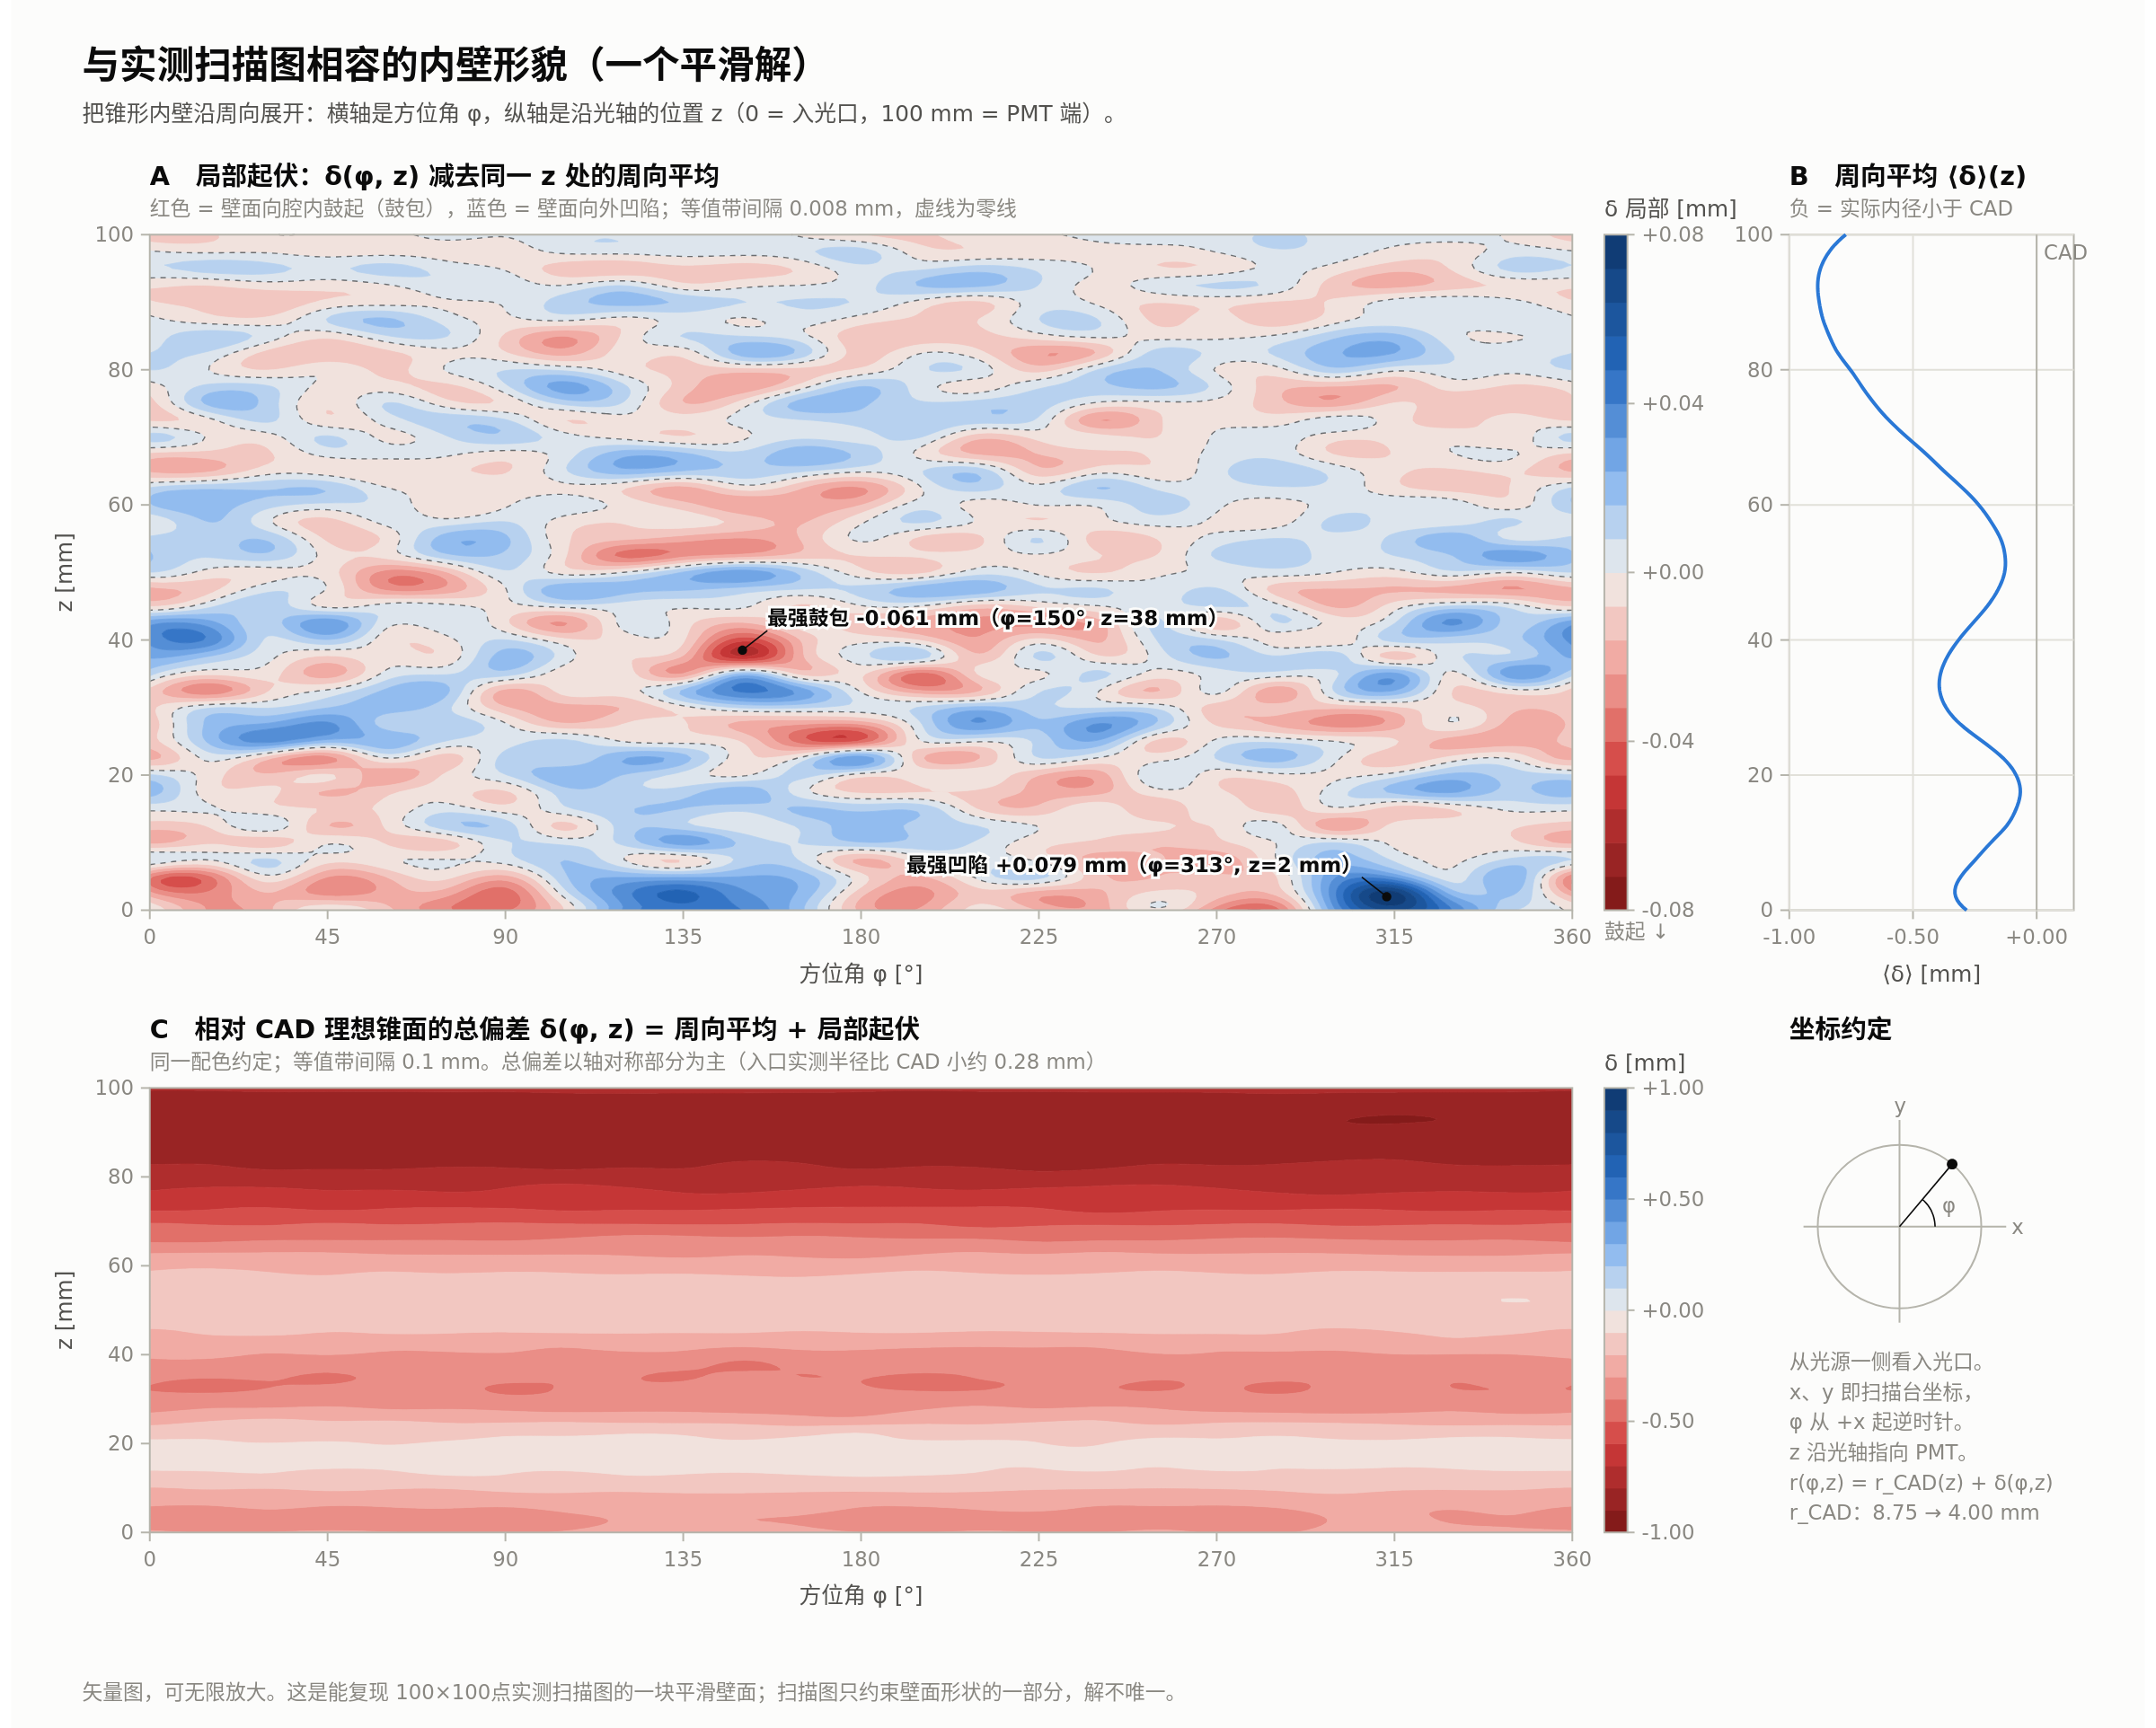
\includegraphics[width=0.88\textwidth]{fig/zh/inner_surface.png}
\caption{内壁形貌图（\texttt{inner\_surface.svg}）。A：局部起伏，即偏差减去其周向平均；B：周向平均；
C：相对 CAD 锥面的总偏差。红色是向腔内鼓起，蓝色是向外凹陷。}\label{fig:wall}
\end{figure}

\begin{figure}[p]
\centering
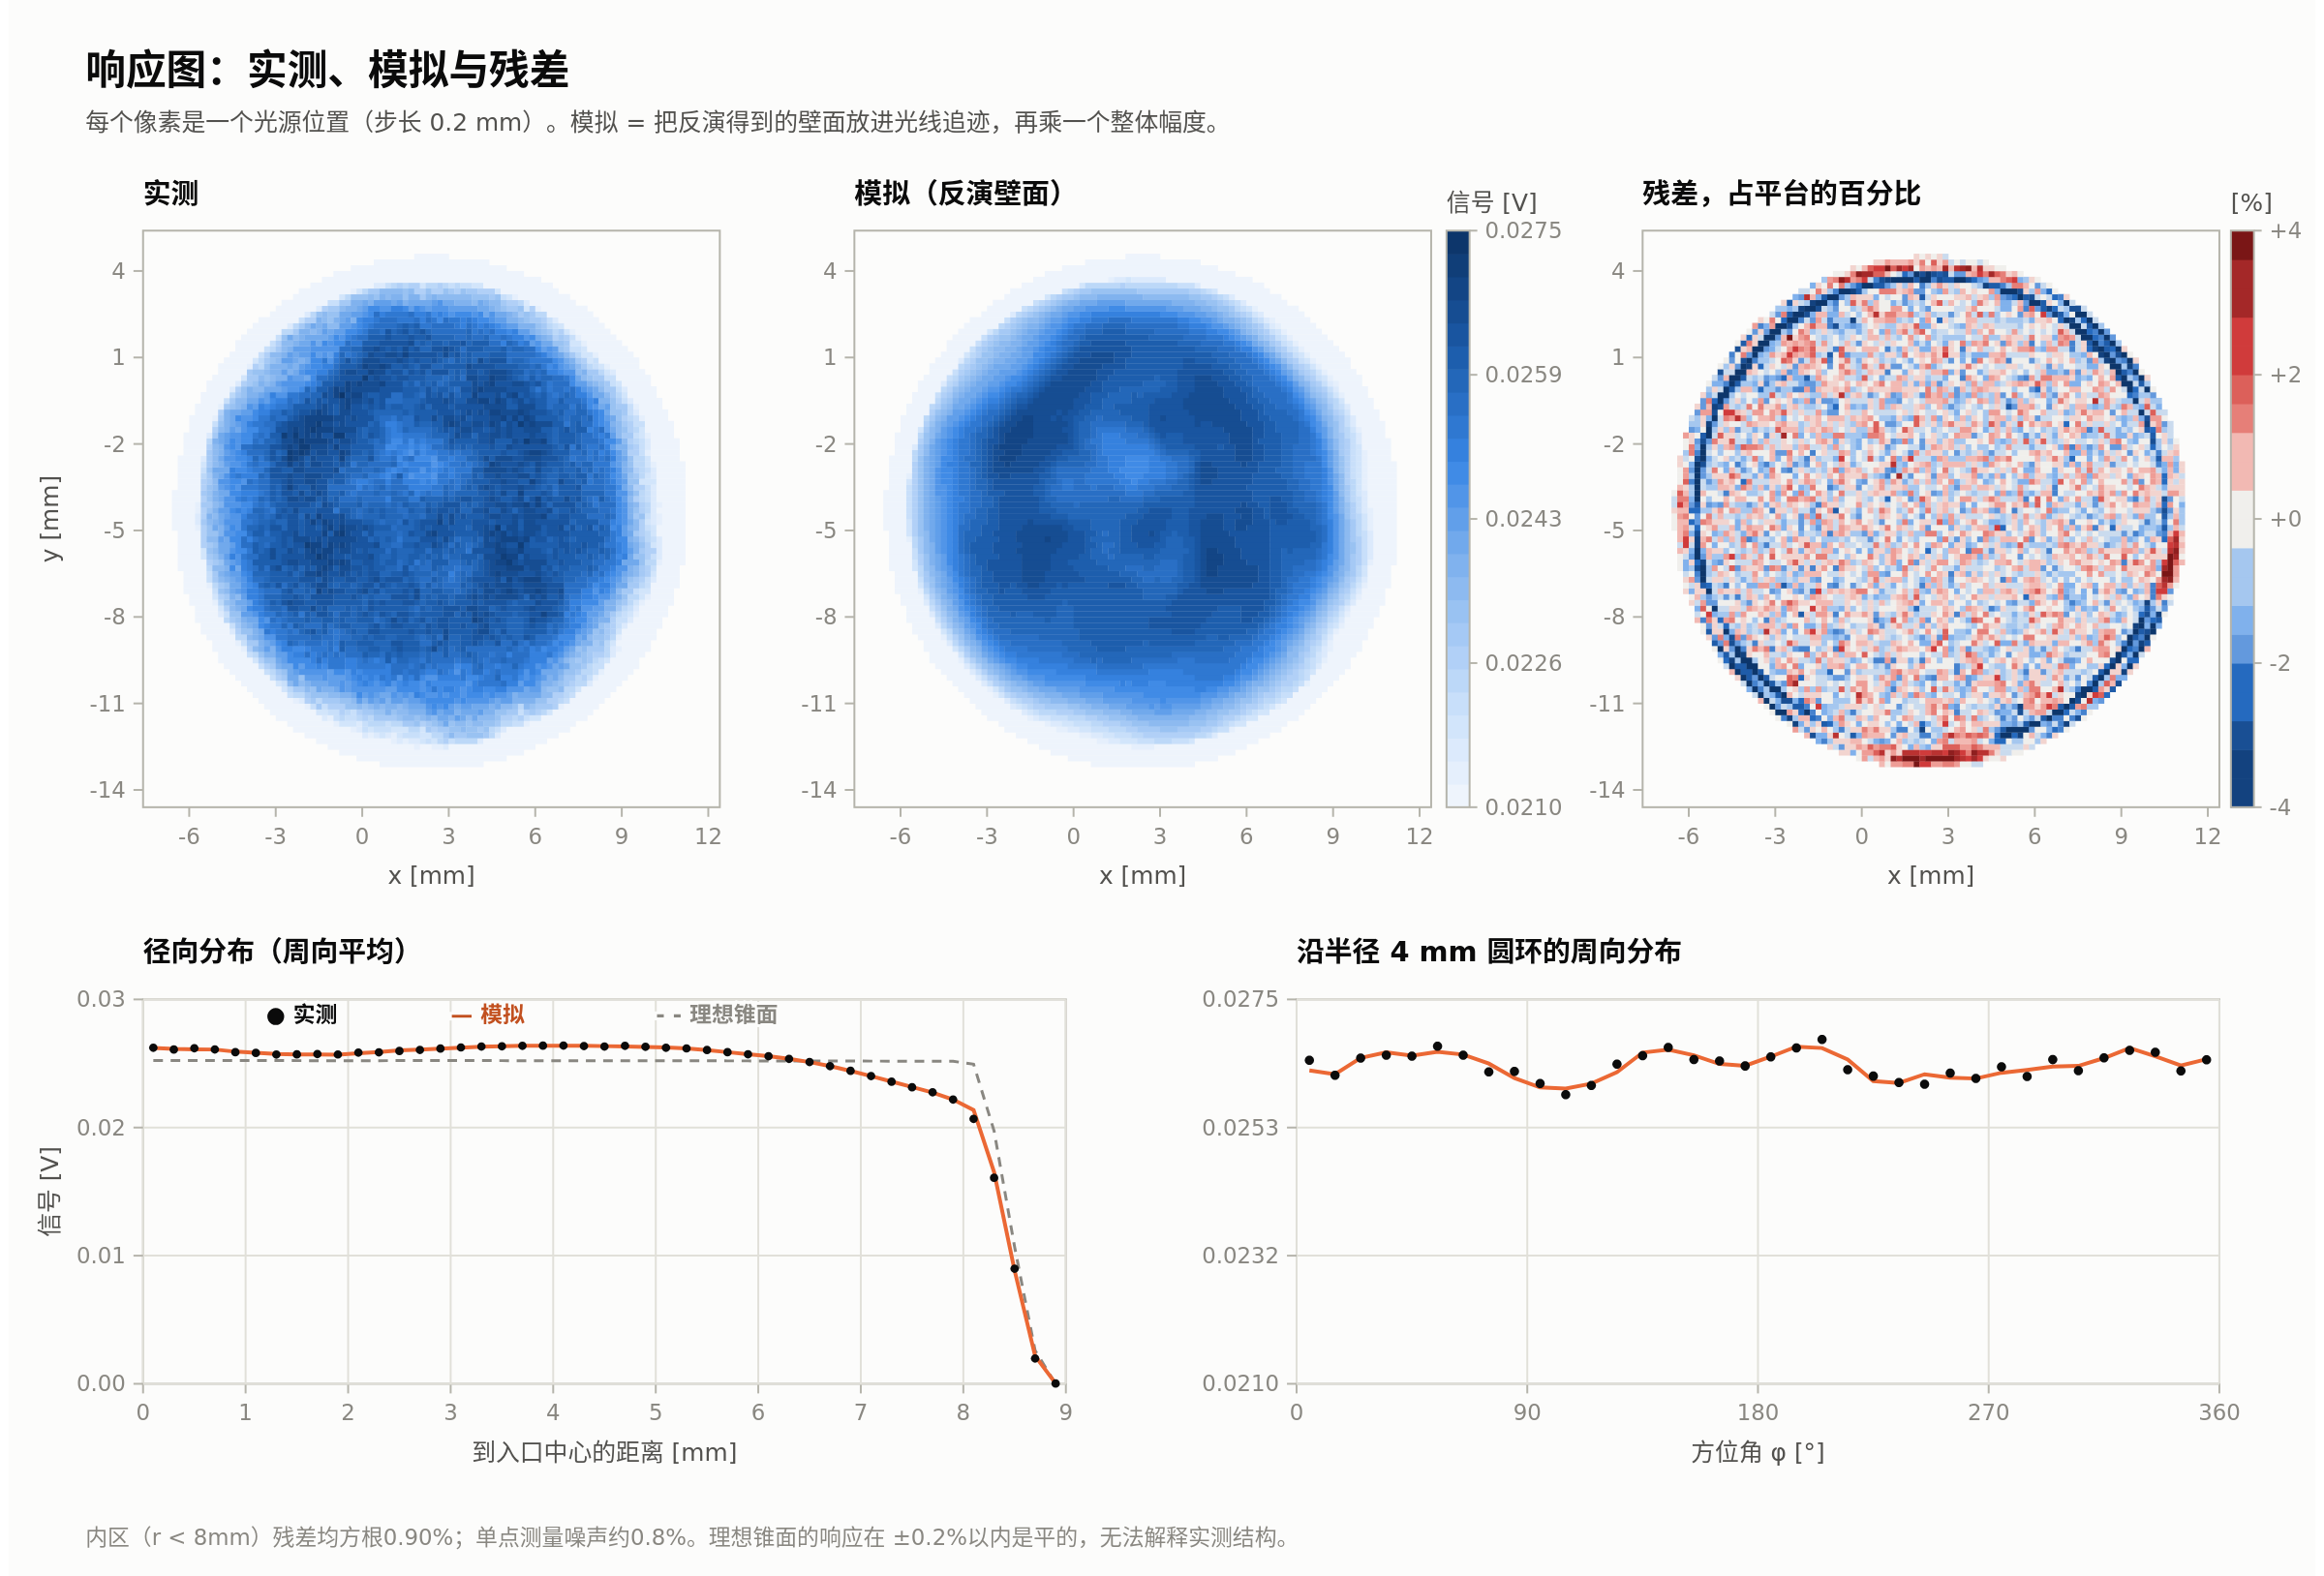
\includegraphics[width=0.88\textwidth]{fig/zh/response_maps.png}
\caption{实测图、模拟图与残差（\texttt{response\_maps.svg}），以及周向平均的径向分布和沿半径 4\,mm
圆环的信号。}\label{fig:maps}
\end{figure}

\clearpage

% ====================================================================== 2
\section{物理与模型}

\subsection{几何与坐标}

长度单位一律为毫米。$z$ 轴是光轴，入口平面为 $z=0$，出口平面（PMT 所在）为 $z=L=100$。CAD 给出的名义
壁面半径是
\[
  r_\mathrm{CAD}(z) = R_1 + (R_2-R_1)\,\frac{z}{L}, \qquad R_1 = 8.75,\quad R_2 = 4.00,
\]
即半角 $2.72^\circ$ 的锥面。实际壁面写成
\[
  r(\varphi,z) = r_\mathrm{CAD}(z) + \delta(\varphi,z).
\]
$\delta<0$ 表示壁面向腔内鼓起（鼓包），$\delta>0$ 表示壁面向外凹陷。

横向坐标 $x,y$ 就是扫描台的坐标轴，原点移到实测的入口孔径中心。方位角 $\varphi$ 从 $+x$ 起逆时针计，
视线方向是从光源一侧看向入口。要把 $\varphi$ 对应到实物，需要知道扫描台坐标轴相对光导的朝向，以及扫的
是模块上四个单元中的哪一个；这两点工具包无从得知。

CAD 文件 \path{data/4cells_17.5mm_8mm_circle_to_circle_100mm-Cut.step} 描述的是含四个相同单元的模块。
每个单元是上述锥面，后接一个直径 16.36\,mm、深 10\,mm 的圆柱形凹槽，用来安装 PMT。进入模拟的只有锥面。

\subsection{光源、壁面与探测器}

\begin{description}[leftmargin=1.6em]
\item[光源] 入口平面上的一个小光斑，像朗伯面一样向前半球发光。光斑是均匀圆斑，半径由扫描图的锐利边缘
量出（随包数据为 \SpotR\,mm）。起点落在孔径之外的光线被挡掉。
\item[壁面] 理想镜面：镜面反射，反射率为 1。反射率也可以设为小于 1（参数 \code{refl}），我们曾在轴对称
拟合中把它作为自由参数：从理想镜面的拟合结果出发、放开反射率后，它走到 \ReflFit，$\chi^2$ 从
\ReflChiFixed{} 降到 \ReflChi（\ReflNpts{} 个点，多一个参数），壁面轮廓的形状变了，幅度仍是同一量级。
反射率与轮廓高度简并，这张扫描图分不开两者，所以结果按理想镜面给出。
\item[探测器] 凡是在壁面以内穿过出口平面 $z=L$ 的光线都计数，不论角度和位置。从入口平面折返出去的光线
算作损失。
\end{description}

光源位于 $(x,y)$ 时的模拟信号为 $A\,T(x,y)$，其中 $T$ 是到达出口的光占全部发射光的比例，$A$ 是由数据
拟合的一个整体幅度（每单位透过率对应的电压）。因此并不使用测量的绝对刻度。

\subsection{理想锥面}
\label{sec:ideal}

对朗伯光源，理想锥面的响应很简单。对入口面积取平均后，透过率严格等于面积比，
\[
  \langle T_\mathrm{ideal}\rangle = \left(\frac{R_2}{R_1}\right)^2 = 0.2090 .
\]
这是光学扩展量守恒的结果：无损的聚光器对朗伯输入的透过率不可能超过面积比；而锥面达到了这个上限，因为从
出口反向发出的每一条光线都能到达入口。

在单个光源位置上，透过率只是近似等于这个值。光线在锥面上反射时，它到锥顶的最近距离保持不变，所以一条
光线能否通过，取决于一个以锥顶为球心、经过出口边缘的球面。而出口是一个平的圆面，不是那块球冠。于是相对
面积比而言，透过率从中心的 $+0.22\,\%$ 缓慢下降到边缘的约 $-0.14\,\%$。本手册的早期版本说响应“严格
平坦”，准确的说法是在 $\pm0.2\,\%$ 以内平坦。

追迹器给出的面积平均值与面积比之差在自检的容许范围内（相对 $2\times10^{-4}$），Geant4 沿半径的结果也与
追迹器一致（第~\ref{sec:validation}~节）。这对反演的意义是：实测图上百分之几的结构不可能来自理想锥面。在
本模型里它被归因于壁面的非理想；模型之外的效应也可能有贡献（见第~\ref{sec:limits}~节）。

\subsection{用 B 样条描述壁面}

$\delta(\varphi,z)$ 是张量积均匀三次 B 样条，
\[
  \delta(\varphi,z) = \sum_{i=0}^{N_\varphi-1}\;\sum_{j=0}^{N_z+2} c_{ij}\,B_i^{(\varphi)}(\varphi)\,B_j^{(z)}(z).
\]
$\varphi$ 方向是周期样条，$N_\varphi=24$ 个节点，位于 $\varphi_i = 2\pi i/N_\varphi$（间隔 $15^\circ$）。
$z$ 方向在 $[0,L]$ 上分 $N_z$ 格，共 $N_z+3$ 个系数；第 $j$ 个系数的中心在 $z_j=(j-1)\,L/N_z$，所以首尾
两个系数各在光导之外一格。最终拟合用 $N_z=40$（每格 2.5\,mm，每个方位 43 个系数），共
$24\times43=1032$ 个壁面参数。样条是 $C^2$ 连续的，表面法向因而连续，这是镜面反射所需要的。

\subsection{光线与壁面求交}
\label{sec:intersection}

光线 $\mathbf p+t\,\mathbf d$ 与壁面的交点，是
$f(t)=\sqrt{x^2+y^2}-r_\mathrm{CAD}(z)-\delta(\varphi,z)$ 由负变正之处。追迹器分三步找到第一个这样的 $t$。
\begin{enumerate}
\item \emph{包络锥面与壁面带。}$\delta$ 介于 $\delta_\mathrm{lo}$ 与 $\delta_\mathrm{hi}$ 之间（在细网格上
取样得到，并留少许余量），所以壁面夹在锥面 $r_\mathrm{CAD}+\delta_\mathrm{lo}$ 与
$r_\mathrm{CAD}+\delta_\mathrm{hi}$ 之间。光线与这两个锥面的交点是二次方程的根。只有落在这层很薄的
\emph{壁面带}里的那段光线才可能碰到壁面；位于内侧锥面以内的那一段用解析的办法直接跳过，剩下最多两个
$t$ 区间需要搜索。
\item \emph{带导数的步进。}在每个区间内以不超过 0.5\,mm 的步长前进，同时取样 $f$ 和它沿光线的导数 $f'$。
$f$ 变号就框住了一个交点。如果相邻两个取样点之间 $f'$ 由正变负，说明 $f$ 在其间有一个极大值；用试位法对
$f'$ 求根找到这个极大值，再检查它的符号。这样，在一步之内进入壁面又离开的掠射交点就不会被漏掉。
\item \emph{Illinois 试位法}在框住的区间内求根，双精度下收敛到 $10^{-10}$\,mm（单精度下为
$2\times10^{-6}$\,mm）。
\end{enumerate}
现在只有当 $f$ 在一个 0.5\,mm 的步长内有两个极值时，交点才可能被漏掉；这要求壁面有远小于样条格距
（轴向 2.5\,mm，弧长方向至少 1\,mm）的结构。

早期版本在整个区间上以 3\,mm 的步长前进，而且只看 $f$ 是否变号；这样的步进可能跨过掠射交点。
\code{test\_grazing\_hit.py} 里保存了一个它漏掉的例子：一条光线在名义锥面以内 11\um{} 处行进，壁面上有一圈
高 11.3\um{} 的环形鼓包，光线在 0.7\,mm 的路程上切入壁面 0.3\um。不过，在随那个版本发表的壁面上，3\,mm
步进、现在的步进和 0.02\,mm 步进对 $2\times10^{7}$ 条光线给出了完全相同的透过率，所以已发表的数字没有
受到影响。
外法向取 $F=r-r_\mathrm{CAD}(z)-\delta(\varphi,z)$ 的梯度，
\[
  \mathbf n \;\propto\; \hat{\mathbf r} \;-\; \frac{1}{r}\frac{\partial\delta}{\partial\varphi}\,\hat{\boldsymbol\varphi}
  \;-\;\Big(\frac{R_2-R_1}{L}+\frac{\partial\delta}{\partial z}\Big)\hat{\mathbf z},
\]
其中的导数由样条解析给出；反射后的方向为 $\mathbf d' = \mathbf d-2(\mathbf d\cdot\mathbf n)\,\mathbf n$。
光线穿过 $z=L$ 即被探测，穿过 $z=0$ 即损失。

\subsection{拟随机光线与公共随机数}

朗伯光源的方向余弦 $(d_x,d_y)$ 在单位圆盘内均匀分布。只对 $\sin\theta\le s_\mathrm{max}$ 的方向取样，
因为更陡的光线不可能到达出口（对拟合得到的壁面，$s_\mathrm{max}=0.5$ 已不损失任何光；流水线取 0.55），
结果再乘以 $s_\mathrm{max}^2$。

光线不是随机的，而是拟随机的。确定一条光线的四个数（两个定方向，两个定光斑内的位置）来自 $R_4$ 加性
递推序列 $u_j(k)=\operatorname{frac}(s_j+k\,g^{-j})$，$j=1\ldots4$，其中 $g=1.1673039782614187$ 是
$x^5=x+1$ 的实根。$1,g^{-1},\ldots,g^{-4}$ 在有理数域上线性无关，所以这些点均匀地填满四维单位立方体。递推
用 32 位整数运算实现，使 CPU 与 GPU 产生完全相同的光线。可选的光斑模糊另外用到两个坐标，取 $\sqrt2-1$ 和
$\sqrt3-1$。每个光源位置有自己的平移量 $s_j$（Cranley--Patterson 平移，由点的序号和种子经哈希得到）。

\emph{本版的更正。}早期版本用的是 $x^4=x+1$ 的根，而它恰好满足 $g^{-3}+g^{-4}=1$。于是定光斑位置的两个
坐标被锁在一起，光斑内的取样点落在一条螺旋线上而不是铺满圆斑，光斑的重心偏移 0.12 个光斑半径，方向逐点
不同。它的后果是模型噪声变大（每点 20\,000 条光线时为 $T$ 的 0.22\,\%，而不是 0.10\,\%），而不是系统
偏差（平均偏移 $4\times10^{-5}$）。现在由 \code{test\_sampler.py} 检查：这些常数之间不存在小系数的整数
关系，任意两个坐标都均匀填满 $32\times32$ 的网格，取样光斑的重心位于光斑中心。

带着这两处修正（第~\ref{sec:intersection}~节的步进和这里的序列），整条流程从头重跑了一遍。拟合质量变化
很小（$\chi^2/N$ 从 1.31 变为 \ChiTwo），但得到的是另一块壁面（第~\ref{sec:prev}~节）。

拟随机光线带来两个性质。
\begin{itemize}
\item $T$ 的噪声比 $1/\sqrt{N}$ 下降得更快：每点 20\,000 条光线时约为 $T$ 的 0.1\,\%，而独立随机
光线约为 1.5\,\%。
\item 种子固定时，响应图是壁面的确定性函数。两块壁面之间的差异于是可以用\emph{公共随机数}来计算：绝大
多数光线在两块壁面里的命运相同，差值的噪声远小于任何一张图自身的噪声。所有有限差分和拟合迭代都依赖这
一点。
\end{itemize}

\subsection{一小块壁面在扫描图上的样子}

位于高度 $z$、方位 $\varphi$ 的一小块形变，并不改变入口面上“正下方”那一点的响应。它改变的是边缘光线的
命运，即那些刚好能到达出口或刚好到不了的光线；对一块给定的壁面，这些光线来自一条细弧上的光源位置。弧的
宽度一般约 0.5\,mm，位置和半径随 $z$ 变化很快：靠近入口的壁面影响紧邻它的孔径边缘，中段的壁面在离中心
几毫米处画出弧和环，靠近出口的壁面给出弥散的环。这幅图像类似层析成像，每个扫描像素对壁面形变沿一条曲线
求和。

这带来两个实际后果：响应非常灵敏（0.03\,mm 量级的形变就能让响应图变化百分之几）；壁面模型在轴向需要
足够细的分辨率（每格 2.5\,mm），才能把弧放到正确的位置。

\subsection{反演}
\label{sec:inversion}

拟合所极小化的目标函数是
\[
  Q(c,A) = \sum_n \frac{\big(d_n-A\,T_n(c)\big)^2}{\sigma^2}
  + \lambda^2\,\lVert P c\rVert^2 + (0.05\,\lambda)^2\,\lVert c-c_\mathrm{base}\rVert^2
  + \sum_i \frac{\big(\delta(\varphi_i,0)-\delta_\mathrm{ap}(\varphi_i)\big)^2}{(0.005\ \mathrm{mm})^2}.
\]
$d_n$ 是拟合半径（默认 8\,mm）以内扣除基线后的扫描值；$\sigma$ 把单点噪声（$2.0\times10^{-4}$\,V）与
模型的蒙特卡洛噪声合在一起；$P$ 对系数沿 $\varphi$ 和 $z$ 取一阶差分（平滑惩罚）；$c_\mathrm{base}$ 是
轴对称的基态壁面；最后一项把 $z=0$ 处的壁面半径约束到由扫描图边缘量出的孔径半径（闭合测试中则约束到
假壁面自己的孔径）。第一项是数据的 $\chi^2$，打印出来的 $\chi^2/N$ 只指这一项。第二、三项惩罚起伏和偏离
基态壁面的程度，用的是样条系数的度量；$Q$ 并不是“在给定拟合容差下壁面表面起伏的均方根”。

$T_n(c)$ 没有解析导数，对单个样条系数直接做有限差分得到的雅可比矩阵又噪声太大。工具包用了两个办法。

\emph{傅里叶模式核。}在轴对称基态附近，某个 $z$ 节点上的周向模式 $\delta c_{ij}=a\cos(m\varphi_i)$
引起的响应，是光源方位角 $\psi$ 的少数几个谐波之和 $\sum_q A_{jmq}(\rho)\cos(q\psi)$，
$q\in\{m,\,N_\varphi-m,\,N_\varphi+m\}$。一次计算扰动整圈壁面，所以信号强而壁面斜率小；向
$\cos(q\psi)$ 投影又把噪声在所有光源方位上平均掉；中心差分消去二阶项。任一单个系数的雅可比由傅里叶合成
和旋转得到。与响应图的精确有限变化相比（第~\ref{sec:jactest}~节），对均方根 10--100\um{} 的非轴对称扰动，
这样的核相关系数为 \JacCorrMin--\JacCorrMax，斜率 \JacSlopeMin--\JacSlopeMax。对周向平均轮廓的变化，核
很差：平缓鼓包的相关系数是 \JacBumpCorrMin--\JacBumpCorrMax，陡的台阶是
\JacStepCorrMin--\JacStepCorrMax。平滑的形变是许多单节点响应大幅相消之后剩下的一小部分，所以单节点核上
百分之几的误差，到了平滑的形状上就成了量级为一的误差。

\emph{带精确残差的阻尼迭代。}每一步 Levenberg--Marquardt 迭代求解带阻尼项 $\mu\lVert\Delta c\rVert^2$
的线性化问题，然后用完整的光线追迹计算真实的 $Q$。$Q$ 下降则接受这一步（并把 $\mu$ 减半），
否则把 $\mu$ 乘以 4 重新求解，最多 8 次。每次试探步实际造成的响应图变化，还通过 Broyden 秩一更新来修正
雅可比。由于残差始终是精确的，不管核有多大误差，每个被接受的步都确实降低了 $Q$。

但这不等于找到了最佳拟合。迭代在连续 8 个阻尼越来越大的试探步都不能降低 $Q$ 时停止；这是一条实用的
停止规则，而不是达到极小的证明。得到的是一个正则化解，它依赖起始壁面、正则化权重和近似的雅可比。此前用
较早版本的代码对随包数据的两次拟合，分别停在 $\chi^2/N=1.48$ 和 1.31；这一次停在 \ChiTwo。

壁面的轴对称部分幅度大（十分之几毫米）且非线性，所以流程先单独拟合轴对称轮廓（Stage A），再做两轮
“算核 + 反演”，第二轮的核在更新后的周向平均壁面附近重新计算。

% ====================================================================== 3
\section{安装}

\subsection{依赖}

\begin{tabularx}{\textwidth}{@{}L{4.6cm}Y@{}}
\toprule
组件 & 用途 \\
\midrule
Python $\ge 3.10$，以及 \code{numpy}、\code{scipy}、\code{matplotlib}、\code{numba}、
\code{contourpy}、\code{pillow} & 全部功能 \\
\code{pyopencl} 与支持 OpenCL 的 GPU & 快速追迹（可选，见 \path{requirements-gpu.txt}；没有时用 \code{LG\_GPU=0}） \\
Geant4 11.x、CMake、C++17 编译器 & \code{g4/} 中的独立交叉验证（可选） \\
Node.js & 光线动画图 \code{ray\_animation.svg}（可选） \\
带 \code{xelatex} 和 \code{ctex} 的 TeX Live & 重新编译本手册（可选） \\
Firefox & 把 SVG 渲染成手册插图（可选） \\
带 \code{systemd} 用户会话的 Linux & 资源限额脚本 \code{tools/run\_limited.sh} \\
\bottomrule
\end{tabularx}

\subsection{Python 环境}

\begin{lstlisting}
git clone <repository url> LGWallRecon
cd LGWallRecon
python3 -m venv .venv
.venv/bin/python -m pip install --upgrade pip
.venv/bin/python -m pip install -r requirements-gpu.txt   # with the GPU tracer (adds pyopencl)
.venv/bin/python -m pip install -r requirements.txt       # or: CPU only
\end{lstlisting}
\path{requirements.txt} 列出只用 CPU 时需要的包；\path{requirements-gpu.txt} 包含前者并加上
\code{pyopencl}，后者需要可用的 OpenCL 驱动。

脚本默认解释器位于包根目录下的 \path{.venv/bin/python}。各个 shell 驱动脚本可以通过变量 \code{PY}
指定别的解释器。

\subsection{GPU（可选，但建议使用）}

只要 \code{pyopencl} 能看到的 OpenCL 设备，追迹器都能用。检查方法：
\begin{lstlisting}
clinfo -l
.venv/bin/python -c "import pyopencl as cl; print([d.name for p in cl.get_platforms() for d in p.get_devices()])"
\end{lstlisting}
开发所用的机器是 AMD Radeon 8060S（Ryzen AI Max+ 395），驱动为 ROCm 7.2；设备在平台
“AMD Accelerated Parallel Processing”下显示为 \code{gfx1151}。AMD 机器上没有 \code{nvidia-smi}，
它也不能说明 GPU 是否可用；请用 \code{clinfo} 或 \code{rocminfo}。

对拟合得到的壁面实测的速度：

\begin{tabularx}{\textwidth}{@{}L{6.2cm}Y@{}}
\toprule
配置 & 每秒追迹的光线数 \\
\midrule
GPU，单精度（默认） & 约 $2.4\times10^{7}$（在机器繁忙时测得） \\
GPU，双精度 & 比单精度慢约 10--30 倍 \\
CPU，双精度（\code{numba}） & 每个核 $10^{5}$ 量级 \\
\bottomrule
\end{tabularx}

也就是说，GPU 版每秒追迹几千万条光线，比这台机器上用全部 CPU 核的版本快大约一个量级。带导数的壁面带步进
（第~\ref{sec:intersection}~节）在 GPU 上比早期版本简单的 3\,mm 步进慢约 1.6 倍，后者曾达到每秒
$3.8\times10^{7}$ 条光线。GPU 内核是单精度的，它对每个光源点给出的结果已与 CPU 双精度版核对
（第~\ref{sec:validation}~节）。没有 GPU 时，加上 \code{LG\_GPU=0} 一切照常运行，只是整条流程要许多个小时
而不是约 50 分钟。

集成显卡与系统共用内存，而 cgroup 的内存上限管不到 GPU 的分配。追迹器把自己的缓冲区控制在几兆字节，
并把任务切成约半秒一片提交，因此既不会耗尽内存，也不会触发驱动的超时复位。

\subsection{Geant4（可选）}

\begin{lstlisting}
source <geant4 prefix>/bin/geant4.sh
cd g4 && mkdir -p build && cd build
cmake .. -DCMAKE_PREFIX_PATH=<geant4 prefix>
make -j4
\end{lstlisting}
生成 \path{g4/build/lgsim}。除标准安装外不需要额外的 Geant4 数据集；程序使用最小物理列表，只含光学光子、
输运和光学边界过程。

% ====================================================================== 4
\section{快速上手}

\begin{lstlisting}
cd LGWallRecon
./run_all.sh
\end{lstlisting}

\code{run\_all.sh} 依次完成：追迹器的三项自检（光线序列、掠射交点、理想锥面，见
第~\ref{sec:validation}~节），量孔径，对 \path{data/scan_summary.csv} 运行反演流程，在拟合壁面上做 GPU
与 CPU 的对比（GPU 开启时），把拟合壁面与此前对同一张扫描图拟合出的壁面相比较（\code{compare\_walls.py}，
第~\ref{sec:prev}~节），导出壁面，绘制中英文图件，生成报告网页。所有耗时的步骤都通过
\path{tools/run_limited.sh} 启动（第~\ref{sec:resources}~节）。各驱动脚本都带 \code{set -euo pipefail}：
任何一步或任何一项自检失败，运行就停止。
\begin{lstlisting}
./run_all.sh --with-checks
\end{lstlisting}
还会运行闭合测试及分辨率分析、互易性检验、雅可比检验、放开镜面反射率的轴对称拟合；装有 Geant4 时再做 Geant4 交叉
验证。

使用 GPU、机器同时忙于其他作业时实测的耗时：从量孔径到最终响应图的整条流程 48 分钟，大部分花在两次核
计算上（每次约 22 分钟）。各项检验合计还要约两小时：闭合测试约 60 分钟，互易性检验约 22 分钟，Geant4（两次
运行，含网格）约 40 分钟。机器空闲时会更快。

结果的位置：

\begin{tabularx}{\textwidth}{@{}L{5.6cm}Y@{}}
\toprule
路径 & 内容 \\
\midrule
\path{results/zh/inner_surface.svg}、\path{results/en/...} & 内壁形貌图（矢量，可缩放） \\
\path{results/<lang>/response_maps.svg} & 实测图、模拟图、残差及分布曲线 \\
\path{results/<lang>/closure.svg} & 闭合测试（运行 \code{closure.sh} 之后） \\
\path{results/<lang>/ray_animation.svg} & 光线传播的侧视动画 \\
\path{results/wall_delta.csv} & $\delta(\varphi,z)$ 数值表，网格 $1^\circ\times0.5$\,mm \\
\path{results/wall_coeffs.json} & B 样条系数 \\
\path{results/numbers.json} & 报告和本手册引用的全部数字 \\
\path{docs/LGWallRecon_report_zh.html}、\path{..._en.html} & 单文件报告网页，含三维演示 \\
\path{out/} & 中间结果 \code{.npz} 和日志 \code{.log}（不纳入版本管理） \\
\bottomrule
\end{tabularx}

如果要手动分步运行，先进入 \path{src/}，脚本里的路径都是相对它写的。
\begin{lstlisting}
cd src
R=../tools/run_limited.sh; PY=../.venv/bin/python
$R $PY edge.py && $R $PY edge_spot.py      # aperture and light spot -> ../out/edge.npz
$R ./pipeline.sh data                      # the reconstruction chain, log in ../out/pipeline_data.log
$R ./make_report.sh ../out/final_data.npz  # exports, figures, report pages
\end{lstlisting}

% ====================================================================== 5
\section{流水线分步说明}
\label{sec:pipeline}

\begin{figure}[H]
\centering
\begin{tikzpicture}[node distance=5mm and 7mm, >=Stealth,
  box/.style={draw=black!55, rounded corners=2pt, align=center, font=\small, inner sep=4pt, minimum height=9mm, text width=27mm},
  io/.style={box, fill=black!6}]
\node[io] (scan) {扫描数据 CSV\\ \footnotesize\ttfamily data/};
\node[box, right=of scan] (edge) {孔径与光斑\\ \footnotesize\ttfamily edge.py, edge\_spot.py};
\node[box, right=of edge] (A) {轴对称轮廓\\ \footnotesize\ttfamily stageA.py};
\node[box, right=of A] (ref) {重采样到 $N_z=40$\\ \footnotesize\ttfamily refine.py};
\node[box, below=9mm of ref] (k1) {算核，第 a 轮\\ \footnotesize\ttfamily kernel\_modes.py};
\node[box, left=of k1] (b1) {反演，第 a 轮\\ \footnotesize\ttfamily stageB.py};
\node[box, left=of b1] (k2) {算核，第 b 轮\\ \footnotesize\ttfamily kernel\_modes.py};
\node[box, left=of k2] (b2) {反演，第 b 轮\\ \footnotesize\ttfamily stageB.py};
\node[box, below=9mm of b2] (fin) {大统计响应图\\ \footnotesize\ttfamily final.py};
\node[io, right=of fin] (out) {壁面、图件、报告\\ \footnotesize\ttfamily make\_report.sh};
\draw[->] (scan) -- (edge); \draw[->] (edge) -- (A); \draw[->] (A) -- (ref); \draw[->] (ref) -- (k1);
\draw[->] (k1) -- (b1); \draw[->] (b1) -- (k2); \draw[->] (k2) -- (b2); \draw[->] (b2) -- (fin); \draw[->] (fin) -- (out);
\end{tikzpicture}
\caption{反演流程。\texttt{pipeline.sh} 执行从 \texttt{stageA.py} 到 \texttt{final.py} 的各步。}
\end{figure}

下面的命令都在 \path{src/} 目录内、通过 \path{../tools/run_limited.sh} 运行。脚本用到的环境变量汇总在
表~\ref{tab:env}。

\subsection{\texttt{edge.py}：入口孔径}

\begin{lstlisting}
python edge.py
\end{lstlisting}
扫描图的边缘很锐，孔径可以直接量出来，不需要光线追迹。脚本取孔径之外很远处（$r>10$\,mm）信号的中位数
作为基线，然后在 48 个方位扇区内拟合径向的边缘轮廓（平台高度、斜率、误差函数形状的边沿）。不断移动中心，
直到边缘半径的 $m=1$ 傅里叶分量为零。输出 \path{../out/edge.npz}，包含中心、基线和边缘半径
$r_\mathrm{ap}(\varphi)$ 的傅里叶系数（$m=0\ldots8$），以及诊断图 \path{../out/edge.png}。

随包数据的平均半径为 \RAp\,mm，比 CAD 的 8.75\,mm 小 \RApDiff\,mm；$m=2$ 和 $m=4$ 分量约 0.03\,mm。

中心的初始猜测和边缘拟合的径向窗口是脚本开头的常数；换一个孔径时要改
（第~\ref{sec:adapt}~节）。

\subsection{\texttt{edge\_spot.py}：光斑}

\begin{lstlisting}
python edge_spot.py
\end{lstlisting}
对全部边缘点做整体拟合，比较高斯光斑和均匀圆斑。圆斑对边缘的描述更好（孔径之外信号没有拖尾）。脚本把
圆斑半径（\SpotR\,mm）和平均孔径半径的一个小修正写入 \path{../out/edge.npz}。之后各步都从这个文件读取
光斑参数。

\subsection{\texttt{stageA.py}：轴对称轮廓}

\begin{lstlisting}
LG_TAG=data python stageA.py 10 fix 3.0
LG_TAG=refl LG_START=../out/A_data.npz python stageA.py 10 refl 3.0
\end{lstlisting}
参数依次为：$z$ 方向的格数 $N_z$（10）；\code{fix} 或 \code{refl}（后者同时拟合镜面反射率）；曲率惩罚
的权重（3.0）。设了 \code{LG\_START=<A\_*.npz>} 时，拟合从此前一次 Stage A 的轮廓出发，反射率从 1 开始，
这样放开反射率的拟合只会比它出发的理想镜面拟合更好，两者的 $\chi^2$ 可以直接比较（第二行；
\code{run\_all.sh --with-checks} 运行的就是它）。反射率上限为 1，对它的导数取向后差分。脚本对扫描图周向平均后的径向分布（$\rho=0.1\ldots7.9$\,mm）拟合一条轴对称的壁面偏移
$\delta_0(z)$ 和幅度，方法是带有限差分和公共随机数的 Levenberg--Marquardt（每个半径 120\,000 条光线）。
$z=0$ 处的半径被约束到实测孔径。输出 \path{../out/A_<tag>.npz} 和一张图。

怎样判断结果：打印出的“data”$\chi^2$ 应比初始值下降一个量级以上，残差图应保持在平台的约 $\pm1\,\%$
以内。但轮廓本身\emph{定不准}：不同的运行会给出明显不同的 $\delta_0(z)$，拟合质量却一样
（第~\ref{sec:limits}~节）。

\subsection{\texttt{refine.py}：沿 $z$ 重采样}

\begin{lstlisting}
python refine.py ../out/A_data.npz 40 ../out/start_data.npz
\end{lstlisting}
把一块壁面改用另一个 $z$ 格数来表示。输入可以是 Stage A 的结果（轮廓被复制到全部 24 个周向节点），也
可以是一块拟合得到的壁面。网格嵌套时（$10\to40$）转换是精确的。

\subsection{\texttt{kernel\_modes.py}：线性响应}

\begin{lstlisting}
python kernel_modes.py ../out/start_data.npz 24 dataa 12000 0.06
\end{lstlisting}
参数依次为：壁面文件（取其周向平均作为基态）、$N_\varphi$、标签、每个光源点的光线数（12\,000）、模式幅度
$a$（mm，0.06；模式 $m$ 用 $\min(a,\,0.18/m)$，以限制高阶模式的壁面斜率；在 \code{pipeline.sh} 里这个幅度
由 \code{LG\_KAMP} 设定）。光源布在极坐标网格上：57 个半径（0.075 至 8.475\,mm）、
半圆上 49 个角度。对 43 个 $z$ 节点中的每一个和每个模式 $m=0\ldots12$，脚本分别用 $+a$ 和 $-a$ 追迹，
保存谐波幅度 $A_{jmq}(\rho)$。输出 \path{../out/kmodes_<tag>.npz}。机器繁忙时 GPU 上约需 22 分钟；每算完一个 $z$
节点打印一行进度。

该模块还提供函数 \code{jacobian(kn, rho, psi)}，由保存的幅度合成任意光源位置上的雅可比矩阵。

\subsection{\texttt{stageB.py}：二维反演}

\begin{lstlisting}
LG_MU=3000 python -u stageB.py dataa dataa 1.0 40 ../out/start_data.npz
\end{lstlisting}
参数依次为：核的标签、输出标签、正则化权重 $\lambda$（1.0）、最大迭代次数（40）、起始壁面。输出
\path{../out/fitB_<out tag>.npz}，每接受一次迭代就重写一次，所以中断的运行可以把这个文件当作起始壁面
接着算。

每次迭代打印一行：
\begin{lstlisting}
it 7: chi2/N 1.518  rms resid 1.016 %  A 0.14979  |delta-base| rms 0.063 max 0.199  rough 11.291
\end{lstlisting}
\begin{itemize}
\item \code{chi2/N}：每个扫描点的数据 $\chi^2$，其中 $\sigma$ = 单点噪声 $\oplus$ 模型噪声。接近 1
表示响应图已拟合到噪声水平。随包数据最终停在 \ChiTwo：还有千分之几、1\,mm 尺度的结构这次拟合没有解释。
闭合测试的假扫描图能达到 \ClChiTwo，说明真值在模型之内时流程可以拟合到噪声水平；至于随包数据在模型之内
是否还有更好的拟合，并不清楚。$\chi^2/N$ 也不是标定过的拟合优度：等效的拟合参数个数是未知的。
\item \code{rms resid}：数据减模型的均方根（不是标准差），以平均信号的百分比表示。
\item \code{|delta-base|}：系数相对基态壁面的均方根和最大值，单位 mm。
\item \code{rough}：$\lVert Pc\rVert^2$ 的值。
\end{itemize}
运行在达到给定迭代次数后结束，或者打印“\code{no improving step; stop}”后结束。这句话的意思是：连续 8 个
阻尼越来越大的试探步（步长小到亚微米）都没能降低目标函数。这就是停止规则，第二轮通常就是这样正常结束的；
它并不证明已经达到极小。如果它在第一次迭代、$\chi^2$ 还很大时就出现，说明阻尼的初值相对壁面的状态太小，
应调大 \code{LG\_MU}（流程中第 a 轮用 3000，第 b 轮用 20\,000）。

设 \code{LG\_VERB=1} 时，每个试探步都会打印步长、线性模型预测的 $\chi^2$、实际达到的 $\chi^2$ 和目标函数。两者
相差很大，说明核已经不能描述当前壁面；应在当前的周向平均壁面附近重新算核。

\subsection{\texttt{final.py}：大统计对比}

\begin{lstlisting}
python final.py ../out/fitB_datab.npz data 40000
\end{lstlisting}
用拟合得到的壁面追迹整个扫描网格（两个种子，用来估计模型噪声），再用半径取实测孔径的理想锥面追迹一遍；
拟合幅度，打印汇总数字，写出 \path{../out/final_<tag>.npz} 和一张诊断 PNG。所有图件和报告都由这个文件
生成。

\subsection{\texttt{pipeline.sh}：整条流程}

\begin{lstlisting}
../tools/run_limited.sh ./pipeline.sh data
\end{lstlisting}
按上面的设置依次运行 Stage A、重采样、两轮“算核 + 反演”和 \code{final.py}。标签决定所有中间文件的名字
（\code{A\_data}、\code{start\_data}、\code{kmodes\_dataa}、\code{fitB\_dataa}、\code{kmodes\_datab}、
\code{fitB\_datab}、\code{final\_data}）。运行前必须先跑过 \code{edge.py} 和 \code{edge\_spot.py}。
设置 \code{LG\_SYNTH=<npz>} 时，流程改用假扫描图而不是实测数据。

脚本先删除同一标签上一次运行留下的文件，把每一步的全部输出写入 \path{../out/pipeline_<tag>.log}，并在第一个
失败的步骤处停止，所以失败的步骤不会被旧文件掩盖。终端上只打印几行摘要。

\subsection{导出、图件与报告}

\begin{tabularx}{\textwidth}{@{}L{6.6cm}Y@{}}
\toprule
命令 & 结果 \\
\midrule
\code{export\_wall.py <final npz> <dir>} & \code{wall\_delta.csv}、\code{wall\_coeffs.json} \\
\code{compare\_walls.py <final npz> <earlier wall\_coeffs json>} & \path{../out/compare_prev.json}：
当前壁面与此前一次拟合的壁面的对比（第~\ref{sec:prev}~节）；由 \code{run\_all.sh} 运行 \\
\code{collect\_numbers.py <final npz> <results dir>} & \code{numbers.json}（已有的各项检验结果也一并
读入，并标明每一项是否属于当前壁面） \\
\code{make\_figures.py <final npz> <dir> <lang>} & \code{inner\_surface.svg}、\code{response\_maps.svg} \\
\code{make\_closure\_fig.py <synth npz> <final npz> <dir> <lang>} & \code{closure.svg}、
\code{closure\_numbers.json} \\
\code{make\_ray\_svg.py <final npz> <dir> <lang>} & \code{ray\_animation.svg}（需要 Node.js） \\
\code{build\_page.py <final npz> <results dir> <out html> <lang> [github] [gitlab]} & 一个单文件报告网页 \\
\code{make\_report.sh [final npz] [github url] [gitlab url]} & 以上全部，中英文各一份；URL 默认是
工具包的主页 \\
\bottomrule
\end{tabularx}

\code{<lang>} 取 \code{zh} 或 \code{en}。图件和网页上显示的所有文字都放在 \path{web/i18n/zh.json} 和
\path{web/i18n/en.json} 里；代码中不含显示用的文字。

\begin{table}[H]
\caption{环境变量。}\label{tab:env}
\begin{tabularx}{\textwidth}{@{}L{2.6cm}L{3.4cm}Y@{}}
\toprule
变量 & 使用者 & 含义（默认值） \\
\midrule
\code{LG\_GPU} & \code{lgtrace.py} & 1：在 GPU 上追迹；0：用 CPU。限额脚本会设为 1；不经限额脚本时默认为 0 \\
\code{LG\_CPUS} & \code{run\_limited.sh} & CPU 核数（按空闲核数自动选取，2--24） \\
\code{LG\_MEM} & \code{run\_limited.sh} & 作业的内存硬上限（\code{6G}） \\
\code{LG\_SCAN} & \code{load\_scan.py} & 扫描数据 CSV 的路径（\path{data/scan_summary.csv}） \\
\code{LG\_SYNTH} & \code{stageA.py}、\code{stageB.py}、\code{final.py}、\code{load\_scan.py} & 含假扫描图及其壁面孔径的 \code{.npz}，用它替换实测数据 \\
\code{LG\_TAG} & \code{stageA.py} & Stage A 输出文件名 \code{A\_<tag>.npz} 中的标签 \\
\code{LG\_START} & \code{stageA.py} & 此前的 \code{A\_*.npz}，以其轮廓为起点（不设：从平直轮廓出发） \\
\code{LG\_RCUT} & \code{stageB.py} & 拟合半径，mm（8.0） \\
\code{LG\_KAMP} & \code{pipeline.sh} & 算核时有限差分的幅度，单位 mm（0.06） \\
\code{LG\_NRAY} & \code{stageB.py} & 每次迭代中每个扫描点的光线数（20\,000） \\
\code{LG\_MU} & \code{stageB.py} & 阻尼的初值（3000） \\
\code{LG\_BROYDEN} & \code{stageB.py} & 1：对雅可比做割线修正（1） \\
\code{LG\_VERB} & \code{stageB.py} & 1：打印每个试探步（0） \\
\code{PY} & 各 shell 驱动脚本 & Python 解释器（\path{../.venv/bin/python}） \\
{\small\code{LG\_GITHUB\_URL}、\code{LG\_GITLAB\_URL}} & \code{make\_report.sh} & 报告网页中显示的仓库地址（工具包的主页） \\
\bottomrule
\end{tabularx}
\end{table}

% ====================================================================== 6
\section{验证工具}
\label{sec:validation}

这些检验回答三个不同的问题：追迹器算得对不对；反演流程能不能找回已知的答案；结果有多依赖假设。
表~\ref{tab:valid} 汇总了随包数据的结果。

\begin{table}[H]
\caption{验证结果。“n/a”表示这项检验没有针对本次反演运行。}\label{tab:valid}
\begin{tabularx}{\textwidth}{@{}L{3.6cm}L{4.3cm}Y@{}}
\toprule
检验 & 结果 & 说明 \\
\midrule
光线序列 & 均匀填满单位立方体 & \code{test\_sampler.py}；不通过时 \code{run\_all.sh} 停止 \\
掠射交点 & 能找到；细步进不改变任何光线 & \code{test\_grazing\_hit.py}；不通过时 \code{run\_all.sh} 停止 \\
理想锥面，追迹器 & 中心 \IdealCentreDev\,\%，边缘 \IdealRimDev\,\% & 相对 $(R_2/R_1)^2$；面积平均与它相差不超过 $2\times10^{-4}$ \\
Geant4，理想锥面 & $T=\GfourIdealT\pm\GfourIdealTErr$ & 与追迹器之比 $\GfourIdealRatio\pm\GfourIdealRatioErr$；\GfourIdealNpoints{} 个点 $\times$ \GfourIdealNphot{} 光子 \\
Geant4，拟合壁面 & 比值 $\GfourRatio\pm\GfourRatioErr$ & \GfourNpoints{} 个点 $\times$ \GfourNphot{} 光子，标准化离散度 \GfourPull \\
GPU 与 CPU & 每个点的结果相同 & 双精度：只差舍入误差；单精度：平均相对差 $\GpuMeanDiff\pm\GpuMeanDiffErr$，离散度 \GpuRmsDiff \\
互易性 & 比值 $\RecipRatio\pm\RecipErr$ & 与 1 相容 \\
雅可比检验 & 相关系数 \JacCorrMin--\JacCorrMax，斜率 \JacSlopeMin--\JacSlopeMax & 均方根 10--100\um{} 的非轴对称扰动。平均轮廓：平缓鼓包 \JacBumpCorrMin--\JacBumpCorrMax，陡台阶 \JacStepCorrMin--\JacStepCorrMax，核在这里很差 \\
闭合测试：响应图 & 残差 \ClMapRms\,\% & 拟合到噪声水平，$\chi^2/N=\ClChiTwo$ \\
闭合测试：壁面 & 相关系数 \ClCorrAll & 真实 \ClRmsTrue\um，恢复 \ClRmsRec\um，两者之差 \ClRmsErr\um（均为均方根） \\
实测图的两次拟合 & 相关系数 \PrevCorr & 较早的壁面拟合到 \PrevRmsEarlier\,\%，当前壁面 \PrevRmsNow\,\%；轮廓相差均方根 \PrevProfDiff\um \\
放开反射率 & $R=\ReflFit$ & 从理想镜面的拟合出发；$\chi^2$ 从 \ReflChiFixed{} 降到 \ReflChi（\ReflNpts{} 个点）；与轮廓简并 \\
\bottomrule
\end{tabularx}
\end{table}

\textbf{一项检验属于哪块壁面。}每项检验的结果文件都带有所用壁面的指纹（样条系数取整后的哈希值；闭合测试和
分辨率分析用的是构造真值所依据的轴对称轮廓的指纹）。\code{collect\_numbers.py} 把它与最终结果的壁面比较，
在 \code{numbers.json} 里给每项检验记下 \code{current: true} 或 \code{false}。报告网页会把此前某次反演
留下的检验明确标出，旧的检验不会被当成新壁面的检验。

\subsection{追迹器的自检}

\begin{lstlisting}
LG_GPU=0 python test_sampler.py        # the quasi-random rays fill their unit cube
LG_GPU=0 python test_grazing_hit.py    # no grazing wall hit is skipped
LG_GPU=0 python test_ideal_cone.py     # ideal cone: area-averaged T = (R2/R1)^2
\end{lstlisting}
每个脚本对每条判据打印 PASS 或 FAIL，有一条不通过就以非零状态退出；\code{run\_all.sh} 一开始就运行这三个
脚本。
\begin{itemize}
\item \code{test\_sampler.py}：光线序列的六个常数之间，$|m_j|\le4$ 的整数组合 $\sum_j m_j\alpha_j$ 与整数的
距离都不小于 $10^{-6}$；任意两个坐标用 65\,536 个点均匀填满 $32\times32$ 的网格；取样圆斑的重心位于圆斑
中心。
\item \code{test\_grazing\_hit.py}：第~\ref{sec:intersection}~节的掠射交点能被找到，CPU 追迹器如此，装有
Node.js 时 \path{web/lgtrace.js} 也如此；在一块随机粗糙壁面上，把步进从正式使用的 0.5\,mm 改成 0.05\,mm，
$3\times10^{6}$ 条光线里没有一条改变命运。
\item \code{test\_ideal\_cone.py}：解析锥面的算法与形变为零的样条算法给出相同的数；按面积加权的平均透过率
与 $(R_2/R_1)^2$ 相差不超过 $2\times10^{-4}$（相对）；中心比它高 $0.22\,\%$，边缘比它低约 $0.14\,\%$
（实测 \IdealCentreDev\,\% 和 \IdealRimDev\,\%）；把发射锥角截在 $\sin\theta=0.7$ 不损失任何光。脚本写出
\path{../out/ideal_cone.json}。
\end{itemize}

\subsection{Geant4}

\code{g4/lgsim} 在一个空腔里追迹光学光子，腔壁是 \code{dielectric\_metal} 型的抛光光学表面，反射率
可设。空腔可以是理想的 \code{G4Cons}，也可以是由壁面网格生成的 \code{G4TessellatedSolid}。
\begin{lstlisting}
lgsim <mesh.txt | ideal> <points.txt> <photons per point> <out.txt> [spot] [smax] [refl] [seed]
\end{lstlisting}
\code{spot} $>0$ 表示高斯光斑的 sigma，$<0$ 表示半径为 $-$\code{spot} 的均匀圆斑（mm）；\code{smax}
与追迹器中一样限制发射锥角。输出每个光源点一行：$x$、$y$、探测到的光子数、发射的光子数、$T$。

\begin{lstlisting}
cd g4
./run_final.sh ../out/fitB_datab.npz [NPROC] [photons per point]
\end{lstlisting}
\code{run\_final.sh} 一次完成两项对比：拟合壁面和理想锥面，光斑和镜面反射率都取自拟合本身。
\code{export\_mesh.py} 把它们写在网格文件旁边（\path{<mesh>.params}：光斑、\code{smax}、反射率），
\code{lgsim} 和 \code{g4\_compare.py} 都读这个文件。

\emph{拟合壁面。}网格有 $1440\times251$ 个顶点，约 72 万个三角面片；每个面片宽 $0.25^\circ$、长 0.4\,mm，
足够细，在目前的精度下看不出面片化的影响。在网格化实体中追迹每个光子约需 10\,ms（理想 \code{G4Cons} 只需
16\,\textmu s），所以 Geant4 只用于核对，不用于拟合。120 个光源点被分成 \code{NPROC} 个列表（默认取空闲
核数，最多 12），每个列表由一个单线程的 \code{lgsim} 进程处理，每个进程约占 0.7\,GB 内存。所有进程都运行
在\emph{同一个}资源 scope 里，合计 \code{NPROC} 个核、\code{NPROC}\,+\,2\,GB 内存
（第~\ref{sec:resources}~节）。脚本检查每个进程的退出状态，并核对所有光源点都有结果返回，否则停止。用 12
个进程时，每点 4000 个光子约需十分钟。

\emph{理想锥面。}\code{G4Cons}，沿半径取 30 个光源点，每点 40\,000 个光子。

\begin{lstlisting}
python g4_compare.py <fit npz | ideal> <params.txt> <g4 out files...>
\end{lstlisting}
\code{g4\_compare.py} 用追迹器以大统计量（每点 400\,000 条光线，在 CPU 上）计算同样的点，把平均透过率
之比及其误差（Geant4 计数的二项分布误差）、标准化离散度（纯统计涨落时为 1）、相关系数和壁面指纹写入
\path{../out/g4_compare.json} 或 \path{../out/g4_ideal.json}。

拟合壁面的结果：比值 $\GfourRatio\pm\GfourRatioErr$，标准化离散度 \GfourPull，相关系数 \GfourCorr。理想
锥面的结果：$T=\GfourIdealT\pm\GfourIdealTErr$，与追迹器之比 $\GfourIdealRatio\pm\GfourIdealRatioErr$。

\subsection{GPU 与 CPU 对比}

\begin{lstlisting}
python test_gpu_vs_cpu.py
\end{lstlisting}
从参与拟合的扫描点中每十个取一个（\GpuNpoints{} 个点，每点 \GpuNray{} 条光线），用同一块壁面、同一个
光斑、同一批光线，分别在 CPU（双精度）、GPU 双精度和 GPU 单精度下追迹。比较的量是每个光源点的透过率，
也就是对该点全部光线的求和，而不是单条光线。
\begin{itemize}
\item 双精度：GPU 在每个点上都必须与 CPU 的值相差不超过两条光线。实际只差舍入误差。
\item 单精度（拟合所用）：平均差必须在其统计误差的四倍以内为零，逐点离散度必须小于 $T$ 的 $10^{-3}$。
实测平均相对差为 $\GpuMeanDiff\pm\GpuMeanDiffErr$，离散度为 \GpuRmsDiff；每点有几条光线的命运改变，这是
边缘光线应有的表现。
\end{itemize}
脚本打印各自的追迹速度，写出 \path{../out/gpu_check.json}，有判据不满足时以非零状态退出。GPU 开启时，
\code{run\_all.sh} 在反演之后运行它。

\subsection{互易性}

\begin{lstlisting}
LG_GPU=0 python test_reciprocity.py ../out/fitB_datab.npz
\end{lstlisting}
对无损的镜面光导，如果两端用同样辐亮度的朗伯光照明，从入口到出口的光通量应等于从出口到入口的光通量。
求交有错，或者法向与表面不自洽，这个等式就会被破坏。脚本在 CPU 上对光滑壁面、两块随机粗糙壁面和拟合
壁面分别做正反两个方向的追迹。每种情形的比值都必须在四个标准差以内与 1 相容，否则脚本以非零状态退出。
拟合壁面的比值为 $\RecipRatio\pm\RecipErr$（写入 \path{../out/recip.json}）。对理想锥面，
两个方向的光通量还都等于出口面积 $\pi R_2^2=50.3$\,mm$^2$，与光学扩展量守恒的要求一致；壁面有形变时，
从出口反向出发的一部分光线会折返，共同的光通量小于出口面积。

\subsection{雅可比检验}
\label{sec:jactest}

\begin{lstlisting}
python test_jacobian.py datab ../out/fitB_datab.npz
\end{lstlisting}
在基态壁面和拟合壁面附近，把核的预测 $J\,\Delta c$ 与响应图的精确变化（每点 200\,000 条光线，公共随机数）
相比较，共七种扰动：五个均方根 0.01--0.1\,mm、不含周向平均的随机平滑场（随机系数经 2 次或 6 次三点平均
平滑，分别称短波长和长波长），以及两个轴对称扰动，一个陡的台阶和一个平缓的鼓包。脚本打印预测变化与精确
变化的相关系数（去掉平均值）和斜率（精确值比预测值，不去平均值）。\code{run\_all.sh --with-checks} 会运行
它，打印的内容保存在 \path{../out/test_jacobian.log}；脚本还写出 \path{../out/jacobian.json}，由
\code{collect\_numbers.py} 收进 \code{numbers.json} 的 \code{jacobian} 块。下表是在本结果的壁面上、用
拟合所用的核（有限差分幅度 60\um）做的那次运行，日志保存为
\path{results/checks/test_jacobian_amp060.log}。

\begin{tabularx}{\textwidth}{@{}Yrrrr@{}}
\toprule
 & \multicolumn{2}{c}{基态壁面} & \multicolumn{2}{c}{拟合壁面} \\
扰动 & 相关系数 & 斜率 & 相关系数 & 斜率 \\
\midrule
均方根 10\um，短波长 & 0.97 & 1.03 & 0.96 & 1.02 \\
均方根 30\um，短波长 & 0.96 & 0.93 & 0.89 & 0.90 \\
均方根 60\um，短波长 & 0.90 & 0.74 & 0.84 & 0.74 \\
均方根 30\um，长波长 & 0.99 & 0.98 & 0.94 & 0.85 \\
均方根 100\um，长波长 & 0.95 & 0.91 & 0.95 & 0.91 \\
轴对称台阶，$z>50$\,mm 处 $+50$\um & 0.27 & 0.95 & 0.13 & 0.93 \\
轴对称鼓包，高 30\um，$z=50$\,mm 处 $\sigma=10$\,mm & 0.50 & 0.30 & 0.44 & 0.30 \\
\bottomrule
\end{tabularx}

怎样读这张表。对非轴对称扰动，核是好的：相关系数 \JacCorrMin--\JacCorrMax，斜率
\JacSlopeMin--\JacSlopeMax。两块壁面附近最差的都是均方根 60\um{} 的短波长场，斜率 0.74：那里响应已经
不再线性。

对周向平均轮廓的变化，核很差。
% M0SMOOTH
对平缓的鼓包，相关系数只有 \JacBumpCorrMin--\JacBumpCorrMax，斜率 0.30；而对这个鼓包的精确响应在高度 5 到 30\um{} 之间是线性的（另行核对过），所以问题出在核上，而不是光导的响应不线性。
对陡的台阶，核把透过率的平均变化算对到 1\,\%，却算不对它的径向分布：相关系数
\JacStepCorrMin--\JacStepCorrMax。

原因是相消。平滑的形变是许多 $z$ 节点之和，各个节点的响应很大而几乎互相抵消：对这个鼓包的响应只有各节点
响应绝对值之和的约 3\,\%。单节点核上百分之几的误差（有限差分的三阶项、蒙特卡罗噪声），到了平滑的形状上
就成了量级为一的误差。

用更小的有限差分幅度做过一次研究，15\um{} 而不是 60\um（\code{kernel\_modes.py ... 0.015}，在流程里是
\code{LG\_KAMP=0.015}；日志为 \path{results/checks/test_jacobian_amp015.log}）：非轴对称场 0.86--1.00，
平缓鼓包 0.66--0.80（斜率 0.62--0.66），台阶 0.26--0.48。有改善，但仍不好。发布的结果\emph{没有}用它
重跑，默认值仍是 60\um。

由此得到的几点。
\begin{itemize}
\item 拟合找平均轮廓方向上的步，效率很低。给出的拟合质量不受影响，因为每个试探步都要经过完整的光线追迹
才决定接受与否（第~\ref{sec:inversion}~节）。这是平均轮廓定不准的又一个原因（第~\ref{sec:limits}~节），
也是拟合可能停在模型所能达到的最佳壁面之前的一个原因。
\item 分辨率分析（第~\ref{sec:resolution}~节）用的是同一套核，它的数字对宽而平滑的形状只是示意性的。
\item 关于不唯一性的两个结论不依赖核。它们都是用完整光线追迹核对过的“存在性”结论：闭合测试中，一块不同于
真值的壁面把假扫描图拟合到了噪声水平；两块不同的壁面对实测扫描图拟合得一样好（第~\ref{sec:prev}~节）。
\end{itemize}

\subsection{闭合测试}

\begin{lstlisting}
../tools/run_limited.sh ./closure.sh 1
python make_closure_fig.py ../out/synth_cl1.npz ../out/final_cl1.npz ../results/zh zh
\end{lstlisting}
\code{make\_synth.py} 构造一块已知的壁面：Stage A 的轮廓加上 7 个高斯形的鼓包和凹陷（高 0.15--0.3\,mm，
沿弧长宽 2--4\,mm，沿轴向长 6--12\,mm）。真值定义在 $48\times23$ 的样条网格上，与拟合所用的
$24\times43$ 网格相比，周向细一倍，轴向粗一倍。真值是平滑的，拟合网格能把它表示到约 0.1\um，所以这个
测试检验的是扫描图能确定什么，而不是网格能表示什么。脚本追迹出一张假扫描图并加上实测的单点噪声。随后
\code{closure.sh} 对它运行 \code{pipeline.sh}，最后做分辨率分析。

反演得到的输入是假壁面自己的入口孔径，正如对真实扫描它得到的是实测孔径：\code{make\_synth.py} 把这个
孔径的傅里叶系数（$m=0\ldots24$）存进假扫描图文件；只要设置了 \code{LG\_SYNTH}，\path{src/load_scan.py}
里的函数 \code{aperture\_fourier} 返回的就是它们。早期版本把实测孔径强加给假壁面，而假壁面的入口与它
相差 38\um（均方根），约束的强度却是 5\um；这等于惩罚了真值，测试并不公平。

\begin{figure}[t]
\centering
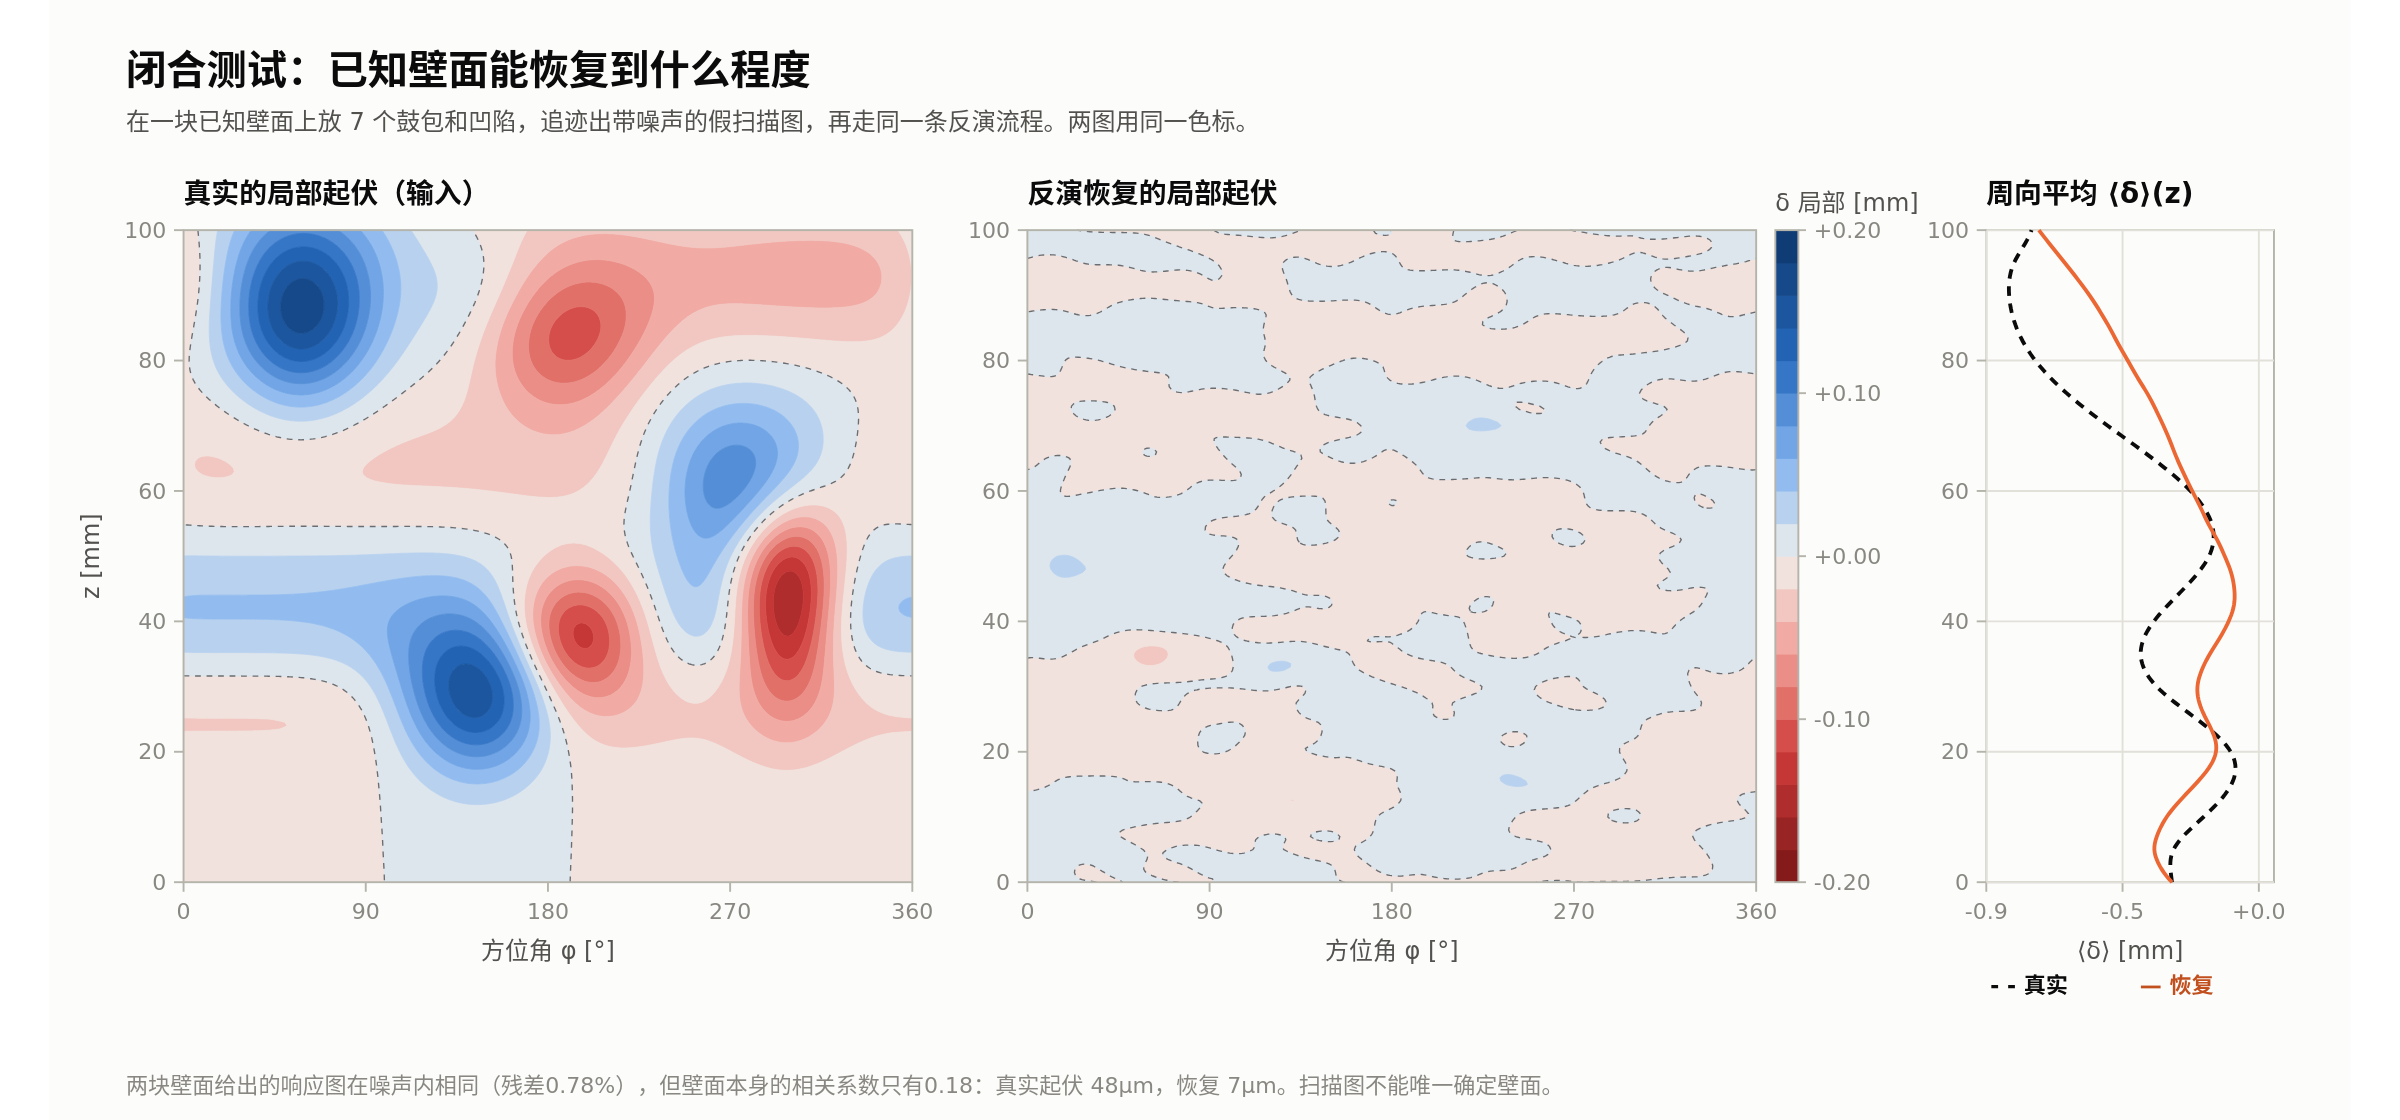
\includegraphics[width=\textwidth]{fig/zh/closure.png}
\caption{闭合测试。左：输入的真实局部起伏；中：由假扫描图恢复出的起伏（同一色标）；右：周向平均轮廓。
两块壁面给出的响应图在噪声范围内相同。}\label{fig:closure}
\end{figure}

结果（图~\ref{fig:closure}）有两层意思，都很重要。假扫描图被复现到了噪声水平：残差 \ClMapRms\,\%，
$\chi^2/N=\ClChiTwo$。这说明真值在模型之内时，流程可以拟合到噪声水平。壁面则是另一回事：真实与恢复的
局部起伏之间只有很弱的相关，相关系数为 \ClCorrAll（完全恢复时为 1），恢复的幅度是 \ClRmsRec\um，而真实值是
\ClRmsTrue\um，两者之差为 \ClRmsErr\um；周向平均轮廓的均方根偏差为 \ClProfErr\um，其中平均偏移
\ClProfBias\um。这些都是均方根而不是标准差：系统偏差计入其中。

\subsection{分辨率分析}
\label{sec:resolution}

\begin{lstlisting}
python study_resolution.py cl1b ../out/synth_cl1.npz ../out/fitB_cl1b.npz
\end{lstlisting}
雅可比矩阵是在轴对称基态壁面附近线性化得到的。先从中投影掉响应图自身的方向（整体幅度在每次拟合里都是
自由参数），再做奇异值分解，把壁面的各种形状组合按它们改变扫描图的强弱排序。扫描图把第 $k$ 个组合的幅度
定到 $\pm\sigma_T/s_k$（一个标准差），$s_k$ 是它的奇异值，$\sigma_T$ 是单个扫描点以透过率为单位的噪声。
表~\ref{tab:res} 对定得最准的前 $k$ 个组合列出：第 $k$ 个组合的这个不确定度（换算成该组合在壁面表面上的
起伏均方根）、测试壁面的真实形变落在其中的比例、在其中真实壁面与恢复壁面的相关系数，以及恢复幅度与真实
幅度之比。

\begin{table}[H]
\centering
\caption{扫描图能确定什么（闭合测试）。对定得最准的前 $k$ 个组合：第 $k$ 个组合幅度的一个标准差不确定度
（换算成表面起伏均方根）、真实壁面形变落在其中的比例、恢复壁面与真实壁面的相关系数、恢复幅度与真实幅度
之比。在 1032 个组合上，奇异值平滑地下降了三个量级。}\label{tab:res}
\begin{tabular}{@{}rrrrr@{}}
\toprule
前 $k$ 个 & 不确定度 [\textmu m] & 比例 [\%] & 相关系数 & 幅度比 \\
\midrule
\ResolutionRows
\bottomrule
\end{tabular}
\end{table}

奇异值是平滑下降的：扫描图“看得见”与“看不见”的组合之间没有清晰的分界，也就不存在一个确定的“可见组合
数”。按明确的截断来说：在前 30 个组合里，恢复的壁面与真实壁面的相关系数为 \ResCThirty，这些组合包含测试
壁面 \ResFThirty\,\% 的形变；前 100 个组合里相关系数为 \ResCHundred（\ResFHundred\,\%），前 150 个里为
\ResCOneFifty（\ResFOneFifty\,\%）。只看相关系数会掩盖幅度上的误差：在前 100 个组合里，恢复的幅度是真实
幅度的 \ResAHundred{} 倍。定得最准的那些组合，幅度被确定到远小于一微米的表面起伏均方根（第 30 个组合
\ResSThirty\um，第 100 个 \ResSHundred\um）；但一块带有宽而缓的鼓包的壁面，其形变只有很少一部分落在这些
组合里。因此有依据的说法是：壁面只在定得最准的大约 100 种组合内被较好地恢复，而它们只占真实形变的约
\ResFHundred\,\%。

四点保留。这里用的雅可比就是核给出的那个，而核对宽而平滑的形状和平均轮廓很差（第~\ref{sec:jactest}~节），
所以表~\ref{tab:res} 的数字只是示意性的，并不精确。这个分析是线性的，线性化的位置是轴对称基态壁面，而不是
拟合得到的壁面。各个组合是按样条系数向量
的度量正交归一的，而不是按壁面表面的度量。一个组合在多大幅度以下看不见取决于幅度本身，所以任何截断 $k$
都是人为的选择。

\subsection{实测扫描图的两次拟合}
\label{sec:prev}

\begin{lstlisting}
python compare_walls.py ../out/final_data.npz ../results/earlier/wall_coeffs_cb81f08.json
\end{lstlisting}
闭合测试是在假扫描图上显示不唯一性，这项检验则是在实测扫描图上。
\path{results/earlier/wall_coeffs_cb81f08.json} 是工具包较早版本（提交 \code{cb81f08}）发布的壁面，
那时追迹器的步进和光线序列还没有修正。脚本用现在的追迹器、孔径和光斑追迹那块壁面（默认每点 20\,000 条
光线，可由第三个参数指定），按 \code{final.py} 的方式拟合幅度，再与当前结果的壁面比较。结果写入
\path{../out/compare_prev.json}，由 \code{collect\_numbers.py} 收进 \code{numbers.json} 的 \code{prev}
块；\code{run\_all.sh} 在流水线之后立即运行它。两块壁面必须在同一张样条网格上。

\begin{tabularx}{\textwidth}{@{}L{3.6cm}L{3.2cm}Y@{}}
\toprule
字段 & 数值 & 含义 \\
\midrule
\code{rms\_earlier}、\code{rms\_now} & \PrevRmsEarlier\,\%、\PrevRmsNow\,\% & 孔径内区实测减模拟的均方根，分别对较早的壁面和当前壁面 \\
\code{map\_diff} & \PrevMapDiff\,\% & 两张模拟图之差的均方根 \\
\code{corr\_local} & \PrevCorr & 局部起伏（去掉周向平均）在整个壁面上的相关系数 \\
\code{bands} & \PrevCorrEntrance；\PrevCorrRest & 同上，沿 $z$ 分成 5 段、每段 20\,mm，从入口到出口 \\
\code{loc\_rms\_earlier}、\code{loc\_rms\_now}、\code{loc\_diff} & \PrevLocRms、\LocRmsOne、\PrevLocDiff\um & 两块壁面各自的局部起伏均方根，以及两者之差的均方根 \\
\code{prof\_diff}、\code{prof\_diff\_max} & \PrevProfDiff、\PrevProfDiffMax\um & 周向平均轮廓之差的均方根和最大值 \\
\bottomrule
\end{tabularx}

怎样读这些数。两块壁面对实测扫描图拟合得一样好，它们的模拟图彼此之间的差别也远小于各自与数据的差别。
如果扫描图能确定壁面，两者就应当一致。实际上它们只在入口后 20\,mm 内一致（相关系数
\PrevCorrEntrance）；再往里，局部起伏不相关甚至相反，两者之差（均方根 \PrevLocDiff\um）比各自的起伏还大，
平均轮廓最多相差 \PrevProfDiffMax\um。这里的相关系数接近 1 只是“壁面被确定”的必要条件而不是充分条件；
现在得到的低值则是直接的证据：就实测数据而言，壁面没有被确定。这两次拟合并不是“所有能拟合的壁面”的
独立抽样（方法相同、正则化相同、起点的取法相同），所以两者之间的差别只是扫描图留下的自由度的下限。

\subsection{其他研究脚本}

\begin{tabularx}{\textwidth}{@{}L{4.7cm}Y@{}}
\toprule
脚本 & 用途 \\
\midrule
\code{study\_deformations.py} & 一组简单测试形变（鼓形、沙漏形、单个鼓包、入口外扩、出口收口）的响应图 \\
\code{study\_reflectivity.py} & 镜面反射率小于 1 时理想锥面的径向分布，与数据对比 \\
\code{study\_launch\_cone.py} & 检查发射角截断 \code{smax} 没有损失被探测的光 \\
\code{look\_data.py} & 原始扫描数据的快速查看图 \\
\bottomrule
\end{tabularx}

% ====================================================================== 7
\section{输出与文件格式}

\subsection{输入的扫描数据}

\path{data/scan_summary.csv} 每个扫描点一行，各列为 \code{idx\_x}、\code{idx\_y}、\code{direction}、
\code{cmd\_x\_mm}、\code{cmd\_y\_mm}、\code{pos\_x\_mm}、\code{pos\_y\_mm}、\code{timestamp}、
\code{n\_events}、\code{n\_saved}、\code{probe\_V}、\code{passed}、\code{acq\_time\_s}。网格序号
\code{idx\_x}、\code{idx\_y} 用来定位每个点；代码使用位置 \code{pos\_x\_mm}、\code{pos\_y\_mm}，信号
\code{probe\_V}（伏）和标志 \code{passed}。网格必须规则且完整。

\subsection{\texttt{out/} 中的中间文件}

\begin{tabularx}{\textwidth}{@{}L{3.5cm}Y@{}}
\toprule
文件 & 数组 \\
\midrule
\code{edge.npz} & \code{cx}、\code{cy} 中心（扫描台坐标）；\code{ped}、\code{ped\_rms} 基线；
\code{fourier[9,2]} $r_\mathrm{ap}(\varphi)$ 的余弦和正弦系数（$m=0\ldots8$）；\code{phi}、\code{r\_edge}、
\code{sigma}、\code{level} 各扇区的边缘拟合；\code{spot\_radius}、\code{dr\_disc} 来自
\code{edge\_spot.py} \\
\code{A\_<tag>.npz} & \code{p} 轮廓系数（若拟合了反射率，也在其中）；\code{NZ}；\code{rho}、
\code{dat}、\code{err}、\code{T}、\code{A} 拟合的径向分布；\code{zz}、\code{d0} 轮廓 $\delta_0(z)$ \\
\code{start\_<tag>.npz} & \code{c[24, NZ+3]}、\code{NZ}、\code{NPHI}、\code{refl} \\
\code{kmodes\_<tag>.npz} & \code{A[nk, 13, 3, nrho]} 谐波幅度；\code{QS[13,3]} 各模式对应的谐波 $q$
（$-1$ 表示未用）；\code{rho}；\code{p} 基态轮廓；\code{T0} 基态响应图；\code{NPHI}、\code{NZ}、
\code{refl} \\
\code{fitB\_<tag>.npz} & \code{c[24, 43]} 拟合得到的系数；\code{base}；\code{A} 幅度；\code{hist}
（每次迭代的 $\chi^2/N$、残差、幅度）；\code{T}、\code{xs}、\code{ys}、\code{dat} 拟合点上的模型、位置
和数据；\code{lam}、\code{NPHI}、\code{NZ}、\code{refl} \\
\code{final\_<tag>.npz} & \code{x}、\code{y} 扫描坐标轴；\code{S[nx,ny]} 扣除基线的数据；\code{M} 模型；
\code{T} 透过率；\code{Mideal} 理想锥面；\code{A}；\code{R} 到中心的距离；\code{cx}、\code{cy}；
\code{phi[361]}、\code{z[201]}、\code{DEL[361,201]} 网格上的壁面；\code{c}；\code{refl}；\code{mc}
模型噪声 \\
\code{synth\_<tag>.npz} & \code{S} 假扫描图；\code{c\_true[48,23]}；\code{bumps}；\code{A}；
\code{fourier[25,2]} 假壁面的孔径；\code{seed}；\code{base\_sha1} 构造真值所依据的轮廓的指纹 \\
{\small\code{pipeline\_<tag>.log}} & \code{pipeline.sh} 每一步的全部输出 \\
\code{ideal\_cone.json}、\code{gpu\_check.json}、\code{recip.json} & \code{test\_ideal\_cone.py}、
\code{test\_gpu\_vs\_cpu.py}、\code{test\_reciprocity.py} 的结果；后两个带有壁面指纹 \code{wall\_sha1} \\
\code{g4\_compare.json}、\code{g4\_ideal.json} & 拟合壁面和理想锥面上 Geant4 与追迹器的对比
（\code{ratio}、\code{ratio\_err}、\code{pull\_rms}、\code{corr}、\code{spot}、\code{refl}、
\code{wall\_sha1}） \\
\code{resolution.json} & 分辨率分析：\code{k}、\code{corr}、\code{amp\_ratio}、\code{frac\_true}、
\code{amin\_um}、\code{amin\_surf\_um}、\code{corr\_all}、\code{base\_sha1} \\
\code{A\_refl.npz} & 放开镜面反射率的 Stage A，从 \code{A\_data.npz} 出发（\code{run\_all.sh --with-checks}） \\
\code{jacobian.json}、\code{test\_jacobian.log} & \code{test\_jacobian.py}：核与响应图精确变化的对比
（第~\ref{sec:jactest}~节）；JSON 文件带有 \code{wall\_sha1}。本手册引用的两次运行的日志保存在
\path{results/checks/} 中 \\
\code{compare\_prev.json} & \code{compare\_walls.py}：当前壁面与此前一次拟合的壁面的对比
（第~\ref{sec:prev}~节），带 \code{wall\_sha1} 和 \code{earlier\_sha1} \\
\bottomrule
\end{tabularx}

\subsection{结果文件}

\code{wall\_delta.csv}：三行注释，然后是各列 \code{phi\_deg}（0--359，步长 1）、\code{z\_mm}（0--100，
步长 0.5）、\code{r\_cad\_mm}、\code{delta\_mm}、\code{delta\_azimuthal\_mean\_mm}、
\code{delta\_local\_mm}。

\code{wall\_coeffs.json}：\code{NPHI}、\code{NZ} 和系数矩阵 \code{c[NPHI][NZ+3]}（mm）。它可以直接喂回
追迹器：
\begin{lstlisting}
import json, numpy as np, lgtrace as lg
c = np.array(json.load(open('../results/wall_coeffs.json'))['c'])
T = lg.transmission([0.0, 2.0], [0.0, -1.0], coeffs=c, nray=20000, smax=0.55, sig=-0.34)
\end{lstlisting}
\code{sig} $<0$ 表示半径为 $-$\code{sig} 的圆斑，\code{sig} $>0$ 表示高斯 sigma；位置相对孔径中心。

工具包较早版本发布的壁面保存在 \path{results/earlier/wall_coeffs_cb81f08.json} 中，文件格式同
上，它是 \code{compare\_walls.py} 的参照。

\code{numbers.json}：壁面指纹（\code{wall\_sha1}），拟合质量（\code{rms}、\code{bias}、\code{rms\_id}、
\code{chi2}、\code{corr}、\code{rms\_ring}、\code{bias\_ring}、\code{ring\_worst}、\code{excess}，以平台的
百分比表示；\code{ring\_worst} 是 8.0 到 8.5\,mm 之间各个 0.1\,mm 圆环上“实测减模拟”的周向平均值中最负的
一个），噪声
（单个扫描点的 \code{noise}、模型响应图的 \code{mc\_noise}，百分比），壁面统计（\code{loc\_rms}、
\code{loc\_min}、\code{loc\_max}，单位 \textmu m；\code{mean\_min}、\code{mean\_max}，单位 mm），孔径
（\code{r\_ap}、\code{spot\_r}），以及做过相应检验后才有的各块：\code{ideal}、\code{g4\_ideal}、
\code{g4}、\code{gpu}、\code{recip}、\code{jacobian}（非轴对称扰动的 \code{corr\_min}、\code{corr\_max}、
\code{slope\_min}、\code{slope\_max}；轴对称扰动的 \code{m0\_step\_corr\_min/max}、
\code{m0\_smooth\_corr\_min/max}、\code{m0\_smooth\_mean\_min/max}）、\code{refl\_fit}、\code{prev}、
\code{closure}、\code{resolution}。所有“rms”都是
均方根，需要时另外给出平均偏差。每一块带有 \code{current}：检验是在本结果的壁面上做的为 true，结果文件是
此前某次反演留下的为 false。

Geant4 网格（\code{mesh.txt}）：第一行是“\code{NPHI NZ}”；之后 \code{NZ} 行，每行是 $z$ 和
$\varphi_i=2\pi i/\code{NPHI}$ 处的 \code{NPHI} 个壁面半径，单位 mm。

% ====================================================================== 8
\section{用于别的光导或别的扫描数据}
\label{sec:adapt}

\textbf{几何。}锥面由三个常数确定，它们出现在四个地方，必须一致：
\begin{itemize}
\item \path{src/lgtrace.py}：\code{R1, R2, L}（以及由它们导出的 \code{SLOPE}）；
\item \path{src/lgcl.py}：OpenCL 源码里的宏 \code{R1}、\code{LEN}、\code{SLOPE}（\code{SLOPE} 是直接
写成数值的）；
\item \path{web/lgtrace.js}：浏览器演示用的 \code{R1, R2, L}；
\item \path{g4/lgsim.cc}：\code{R1, R2, LEN}；如果光导大得多，还要改 world 盒子和两端光子吸收体的尺寸。
\end{itemize}
\code{export\_wall.py} 和 \code{make\_ray\_svg.py} 里也直接写了 $r_\mathrm{CAD}=8.75-0.0475\,z$。如果
形状不是直锥，需要在函数 \code{\_f}、\code{\_fg} 和包络锥面的求根区间里换一个参考面；B 样条部分可以原样沿用。

\textbf{扫描数据。}任何规则的矩形网格都可以。要么提供列名相同的 CSV 并用 \code{LG\_SCAN} 指向它，要么
修改 \path{src/load_scan.py} 里的 \code{load()}；它必须返回坐标轴 \code{x}、\code{y} 和信号
\code{V[ix, iy]}。在 \path{src/edge.py} 里设置中心的初始猜测，以及求基线（$r>10$）和拟合边缘
（$7.6<r<9.6$）所用的径向窗口。

\textbf{拟合半径。}\code{LG\_RCUT}（8.0\,mm）离孔径边缘的距离必须大于光斑半径，保证拟合点上的光斑不被
孔径切到。\code{kernel\_modes.py} 里的极坐标网格（57 个半径，间隔 0.15\,mm）必须覆盖它。

\textbf{发射锥角。}\code{smax} 必须大于任何被探测光线的 $\sin\theta$，大致是 $R_2/R_1$ 再加一点余量，
可用 \path{study_launch_cone.py} 检查。取得太小会不声不响地丢光，取得太大只是多花时间。

\textbf{壁面的分辨率。}$N_\varphi$ 是 \code{kernel\_modes.py} 的参数，\code{refine.py} 对 Stage A 的
输入固定写出 24 个周向节点；$N_z$ 是 \code{refine.py} 的第二个参数。网格更细可以分辨更细的弧，但也带来
更多约束不住的参数；计算量与核的计算次数 $N_z\times(N_\varphi/2+1)$ 成正比。

\textbf{正则化。}$\lambda$ 是 \code{stageB.py} 的第三个参数。在阻尼迭代下结果对它的依赖很弱：拟合
本来就停留在起始壁面附近。想看先验的影响，应当换起始壁面，而不是改 $\lambda$。

\textbf{噪声与统计量。}扫描的单点噪声（\code{stageB.py} 里的 \code{SIGD}，\code{final.py} 和
\code{collect\_numbers.py} 也用到）对随包数据是 $2.0\times10^{-4}$\,V；新数据要由平台区的高通残差重新
估计。每点光线数：算核 12\,000，每次迭代 20\,000，最终响应图 40\,000。减半大致使运行时间减半，模型噪声
增大 30--40\,\%。

% ====================================================================== 9
\section{局限与解读}
\label{sec:limits}

\textbf{解不唯一。}不同的壁面可以给出在噪声范围内相同的响应图。对实测扫描图的两次拟合复现得一样好
（\PrevRmsEarlier\,\% 和 \PrevRmsNow\,\%），得到的两块壁面却只在入口附近一致：整体相关系数 \PrevCorr，
入口后 20\,mm 内为 \PrevCorrEntrance（第~\ref{sec:prev}~节）。闭合测试中，真实壁面只在扫描图定得最准的
大约 100 种形状组合内被较好地恢复（相关系数 \ResCHundred），而这些组合只占真实形变的 \ResFHundred\,\%
（表~\ref{tab:res}）；一块带宽而缓、高 0.15--0.3\,mm 鼓包的壁面（均方根 \ClRmsTrue\um）与恢复出来的
均方根 \ClRmsRec\um{} 的壁面，对同一张假扫描图拟合得一样好。这里给出的是一个正则化解：拟合对起伏加了惩罚，阻尼迭代又停留在轴对称的起始
壁面附近，所以它倾向于平滑的壁面。但没有证明它是能拟合数据的壁面里起伏最少的一块，因为停止规则不证明
达到了极小，$Q$ 也不是表面起伏的均方根。\LocRms\um{} 的局部起伏均方根说明，很小的起伏就足以解释这张
扫描图。它既不是对真实壁面起伏的估计，也不能保证真实壁面的起伏不会比它小：部分结构可能来自反射率或
探测器的不均匀，而不是几何。

\textbf{周向平均轮廓定不准。}它与整体信号幅度、出口半径和镜面反射率高度简并，不同的拟合给出不同的轮廓。
现在这条轮廓与较早那块壁面的轮廓相差均方根 \PrevProfDiff\um，最大 \PrevProfDiffMax\um，两者的拟合质量
却相同；闭合测试中恢复的轮廓误差均方根为 \ClProfErr\um；放开反射率时，轴对称拟合走到 $R=\ReflFit$ 和
另一条轮廓。线性核对平均轮廓的变化很差（第~\ref{sec:jactest}~节），所以拟合找这类步的效率很低。各次拟合共同的只有入口半径（\RAp\,mm，由扫描图边缘直接量出）和“内腔全长都比 CAD 细”这一点。
局部起伏均方根这一次是 \LocRmsOne\um，较早那块壁面是 \PrevLocRms\um，更早一次从另一个起点出发的拟合是
44\um；它们都能把扫描图复现到 1\,\% 左右。

\textbf{一切都算在几何头上。}按假设，镜面反射率为 1，PMT 的响应对位置和角度都均匀，光源是理想的朗伯
圆斑。实际的反射率不均、反射膜的接缝、灰尘、光阴极不均匀，都会被当成壁面的起伏。

\textbf{没有解释的结构。}对随包数据的拟合停在 $\chi^2/N=\ChiTwo$ 而不是 1：还有千分之几、1\,mm 尺度
的相关结构这次拟合没有解释。闭合测试表明，真值在模型之内时流程可以拟合到噪声水平；但它不能说明对随包数据
的这次拟合已经是模型所能达到的最好结果：此前用较早版本的代码对同一份数据的两次拟合分别停在 $\chi^2/N=1.48$ 和 1.31，可见
这个值依赖起点、设置和代码版本。剩余的部分可能是模型（平滑壁面、理想镜面、均匀探测器）之外的结构，也可能是优化没有
走到头，或者两者都有。$\chi^2/N$ 不是标定过的拟合优度，因为等效的拟合参数个数未知。

\textbf{入口边沿。}在 $r=8.0$\,mm 到孔径边缘（\RAp\,mm）之间，实测低于模型。8.0 到 8.5\,mm 的环带里，
逐点残差的均方根约 \RmsRing\,\%，平均值为平台的 \BiasRing\,\%；最差的 0.1\,mm 圆环上周向平均值达到
\RingWorst\,\%。
实测信号在孔径内侧比模型掉得早，外侧却没有拖尾，像是入口边沿有一条约 0.1\,mm 宽的损失带（倒角，或者
反射膜没有贴到边）。这小于模型的分辨率，这一圈没有参与拟合。

\textbf{分辨率。}偏差场的格距是轴向 2.5\,mm、周向 $15^\circ$（入口处弧长 2.2\,mm，出口处 1.0\,mm）。
更细的结构被平滑掉。

\textbf{方位角的对应。}$\varphi$ 跟随扫描台坐标轴。图与实物是否互为镜像，取决于扫描台的朝向。

\textbf{怎样才能定出真实壁面。}需要独立的信息，每一种都会多约束一批形状组合：
\begin{itemize}
\item 用准直光束在若干入射角下各扫一遍（每个角度挑出不同的光线族，而漫射光源把它们全部平均掉了）；
\item 在出口处做角分辨或位置分辨的读出，而不是只用一个积分的 PMT；
\item 从出口一侧反向扫描；
\item 直接用轮廓仪测内壁，或在几个高度上用三坐标测内径，以确定周向平均。
\end{itemize}
在采集数据之前，可以对设想中的附加测量做一次模拟，重复分辨率分析（\code{study\_resolution.py}），看它
能多让多少种组合变得可见。

% ====================================================================== 10
\section{常见问题}

\trouble{GPU 追迹器启动时报 \code{IndexError} 或找不到设备}{\code{pyopencl} 没有找到 GPU 设备。检查
\code{clinfo -l}；确认用户在 \code{render} 和 \code{video} 组里；AMD 机器上确认已安装 ROCm 的 OpenCL
ICD。不用 GPU 时设 \code{LG\_GPU=0}。}
\trouble{运行时桌面卡顿，或 GPU 驱动复位}{追迹器每次提交约 0.6\,s 的任务片
（\code{lgcl.transmission} 的 \code{slice\_s}）。如果 GPU 还要供交互使用，把它调小。同一时间只跑一个
GPU 作业。}
\trouble{修改 \code{lgtrace.py} 后结果变了，或 \code{numba} 报缓存函数的错误}{删除
\path{src/__pycache__}。编译好的函数缓存在那里，下次运行会重新生成（几秒钟）。}
\trouble{驱动脚本报“step failed”或打印 FAIL 后停止}{各 shell 驱动脚本在第一个失败的步骤或自检处停止。
\code{pipeline.sh} 会打印 \path{out/pipeline_<tag>.log} 的末尾；该步骤的完整输出在这个文件里。}
\trouble{作业以退出码 137 结束，或显示“Killed”}{它超过了限额脚本的内存上限。流水线需要的内存不到
1\,GB；用 72 万面片网格的 Geant4 作业约 0.7\,GB。只有确知作业需要更多内存时，才用 \code{LG\_MEM=12G}
调高上限。}
\trouble{第一次迭代就出现“no improving step; stop”}{见第~\ref{sec:pipeline}~节：调大 \code{LG\_MU}，
或在当前壁面附近重新算核。在一次运行的末尾出现这句话是正常的停止规则。}
\trouble{\code{stageB.py} 停止了，但最终的 $\chi^2$ 更高}{\code{final.py} 用的是另一个种子和更多的
光线；$\chi^2/N$ 相差百分之几属于蒙特卡洛噪声。差别更大则说明拟合跟着自己那批光线的噪声走了；调大
\code{LG\_NRAY}。}
\trouble{手册插图是空白的，或 Firefox 无法启动}{有别的 Firefox 在使用同一个配置目录。
\code{make\_manual\_figs.sh} 在 \path{docs/manual/.ffprofile} 里保存自己的配置；删除该目录后重新运行。}
\trouble{Geant4：“Overlapping daughter with mother volume”}{\code{lgsim.cc} 里的 world 盒子必须包住
空腔和两端的光子吸收体；光导长于 100\,mm 时要把它加大。}
\trouble{Geant4：“Particle e- without a Process Manager”}{单独注册 \code{G4OpticalPhysics} 时会出现
这个错误。请保留 \code{lgsim.cc} 里的最小物理列表：只构造光学光子，加上输运和光学边界过程
（\code{G4OpBoundaryProcess}）。}
\trouble{Geant4 非常慢}{在网格化实体中追迹，每个光子约 10\,ms，面片数在 18 万到 72 万之间时差别不大。
用少量的点、每点几千个光子，分成多个进程并行。}

% ====================================================================== 11
\section{资源使用策略：\texttt{tools/run\_limited.sh}}
\label{sec:resources}

开发所用的机器是多人共用的，所以每个耗时或并行的作业都通过一个限额脚本启动，使它不会耗尽内存，并把 CPU
让给别的任务。
\begin{lstlisting}
tools/run_limited.sh <command> [arguments...]
tools/run_limited.sh --cores        # print the number of cores a job would get now
\end{lstlisting}
\begin{itemize}
\item 每调用一次，命令就运行在一个临时的 \code{systemd} 用户 scope 里，设有 \code{MemoryMax}（默认
6\,GB）且禁用交换分区：超限的作业会被杀掉。
\item 核数在作业启动时确定：全部核数减去正被别的任务占用的核数，再减去 4 个余量，限制在 2 到 24 之间。
它同时决定 scope 的 CPU 配额，以及 \code{numba}、OpenMP 和 BLAS 的线程数。
\item 作业以 \code{nice 19}、空闲 I/O 优先级和 CPU 权重 10 运行，其他任务优先得到 CPU。
\item 脚本导出 \code{LG\_GPU=1}，所以追迹默认在 GPU 上进行，除非另外给出 \code{LG\_GPU=0}。
\end{itemize}
可在命令前覆盖：\code{LG\_MEM=12G}、\code{LG\_CPUS=8}、\code{LG\_GPU=0}。在没有 \code{systemd} 用户
会话的机器上，直接运行各条命令，并手动设置 \code{LG\_GPU=1} 和 \code{NUMBA\_NUM\_THREADS}。

限额脚本做不到的事。限额只对一次调用有效：并排启动的作业各有各的 scope 和各自的限额，所以需要总量上限
的并行任务，必须在\emph{同一次}调用内部启动；\code{g4/run\_final.sh} 对它的 Geant4 进程就是这样做的。
另外，cgroup 的内存上限管不到 GPU 的分配，GPU 不在 cgroup 的统计之内。因此追迹器自我约束：主机端缓冲区
只有几兆字节，任务片不到一秒。同一时间只跑一个 GPU 作业。

% ====================================================================== 12
\section{作者、联系方式、许可证与引用}

LGWallRecon 的作者是李衡讷（Hengne Li），华南师范大学。

联系方式：\code{Hengne.Li@cern.ch}，\code{Hengne.Li@m.scnu.edu.cn}。

代码仓库：
\begin{itemize}
\item GitHub：\GithubURL
\item GitLab（SCNU 组）：\GitlabURL
\end{itemize}

许可证：LGWallRecon 以 MIT 许可证发布，Copyright (c) 2026 Hengne Li (李衡讷)。
你可以使用、复制、修改和再分发它，包括 \path{data/} 中的实测扫描数据和 CAD 文件，
只需保留版权声明和许可声明。软件不附带任何担保。许可证全文见仓库根目录的 \path{LICENSE} 文件。

引用本工具包时请写：
\begin{quote}
Hengne Li, \emph{LGWallRecon: light-guide inner-wall reconstruction from an entrance-face scan},
software, 2026.\\
\GithubURL
\end{quote}

引用用它得到的结果时，请说明模型的假设（理想镜面、均匀探测器、朗伯光源），并说明重建出的壁面是一个
解不唯一的反问题的一个正则化解。

\end{document}
